\documentclass[[12pt,DIV14,BCOR12mm,a4paper,footexclude,headinclude,halfparskip-,twoside,openright,cleardoubleempty,idxtotoc,bibtotoc]{article}

\usepackage[textwidth=16cm,textheight=26cm]{geometry}
%\usepackage[top=3cm,bottom=2]{geometry}


\usepackage{graphicx}
\usepackage[english]{babel}
%\usepackage[font={small}]{caption}
\usepackage[font=small,format=hang]{subcaption}
\usepackage[font=small,format=hang]{caption}
%\usepackage[format=hang]{caption}       % for hanging captions
%\usepackage{subfig}                     % for subfigures
\usepackage{wrapfig}                    % for figures floating in text, alternatively you can use >>floatflt<<
\usepackage{pifont}
\usepackage{framed}


\usepackage{tikz}
\usetikzlibrary{arrows,positioning,shapes.geometric, calc, shadows, decorations.pathreplacing, patterns, hobby}


\usepackage{hyperref}

\usepackage{algorithm}
\usepackage[noend]{algpseudocode}
\usepackage{dirtree}
\usepackage{epstopdf}
\usepackage{tikz}
\usepackage{anyfontsize}
\usepackage{scalefnt}
\makeatletter
\def\BState{\State\hskip-\ALG@thistlm}
\makeatother
\usepackage{psfrag}
\usepackage{epsfig}
\usepackage{multirow}
\usepackage{pgf} 
\usepackage{pgffor} 
\usepgflibrary{plothandlers} 


%\usepackage[table]{xcolor}

%%%%%%%%%%%%%%%%%%%%%%%%%%%%%%%




\begin{document}

\title{The Livius Documentation}
\author{Author: Parnia Bahar}

\maketitle

\begin{abstract}
This Documentation serves as a short description for all required knowledge and previous works regarding the Livius project in Max-Planck Institute of intelligent system, Empirical Inference department. The main aim of the work is to automatically create an appropriate layout for online courses and lectures.  In this case, a proper framework should be composed of both the lecture slides/board and the speaker/teacher. To this aim, computer vision and machine learning  based algorithms are applied to detect the slides and track the person of interest.
\end{abstract}

\section{Introduction}

There are many advantages to online and computer-based learning when compared to traditional face-to-face courses and lectures, however, there are a few disadvantages as well.
Online courses are great for self-motivated individuals who want to learn new skills and advance their careers and their knowledge without attending in the college or university. Getting education online will also save tons of money. Although some would argue that online education is only an awesome alternative to traditional education because of the savings and convenience, there are actually many other advantages. Only online education fully integrates itself into today’s educational technology. It is also more efficient for fast and especially motivated learners and offers skills that lack resources in traditional education despite high demand from employers. 

Class work can be scheduled around work and family.
It reduces travel time and travel costs for off-campus students.
Students may have the option to select learning materials that meets their level of knowledge and interest.
Students can study anywhere they have access to a computer and Internet connection.
Self-paced learning modules allow students to work at their own pace.
Flexibility to join discussions in the bulletin board threaded discussion areas at any hour, or visit with classmates and instructors remotely in chat rooms.
Instructors and students both report e-Learning fosters more interaction among students and instructors than in large lecture courses.
e-Learning can accommodate different learning styles and facilitate learning through a variety of activities. Develops knowledge of the Internet and computers skills that will help learners throughout their lives and careers.
Successfully completing online or computer-based courses builds self-knowledge and self-confidence and encourages students to take responsibility for their learning.
Learners can test out of or skim over materials already mastered and concentrate efforts in mastering areas containing new. information and/or skills \cite{IOWA:Online}.
In this case, the demand of taking online classes is increasing and there are many universities and educational organizations which offer free online courses. Therefore, there are some attempts to provide students and online-audiences with a high quality and interesting videos so that they can follow all of the course material in a desire manner. For this purpose, besides the slides/board including the taught sections, it is worthy to watch the speaker/teacher's reactions during the class.



\subsection{The Framework }

As it was mentioned, we try to have both speaker and slide parts in a single video and then broadcast it on the net. In summer school 2013, there were some efforts to do it manually or to make it by helping of two cameras. One camera has been concentrated on the slides to record the video and another one has been manually controlled by a person to track the speaker during the lecture. But the synchronization of two cameras is challenging and recording the videos for speakers' movements is time consuming. Thus, a high resolution 4k camera is used in Livius project to record the lectures and by means of image analysis, computer vision and machine learning approaches, one detects not only the slides, but also tracks the speaker in an intelligent manner as automatic as possible.


One can see the whole framework of the project in the figure \ref{fig_framework}. The whole project can be divided into three major tasks. The first one is video processing and it is related to all algorithms, pre- and post-processing steps for slide detection and speaker tracking. Here, the processing tasks can be done either on the video file itself or on the separate frames. The second one can be called video editing and it includes all necessary works for the codecs of the video, the final layout, the background image, the logo and concatenating all together to form the final version of the video. The third part is audio processing and it refers to all works on audio signal either stereo or mono. Finally, the improved version of audio signal will be reconnected and synchronized with video file to create the final video with desired layout (see figure \ref{fig_layout}). 


\subsection{Output video layout}

In order to broadcast the final video, the full HD size is used. The final video size to stream is 1920x1320. Figure \ref{fig_layout} depicts the final layout and the first page and background images.


\begin{figure}[ht]
\resizebox{1\linewidth}{!}{
\pgfdeclarelayer{background}
\pgfdeclarelayer{foreground}
\pgfsetlayers{background,main,foreground}

\begin{tikzpicture}[>=latex']

\tikzset{block/.style={
      rectangle,
      draw=blue,
      thick,
      fill=gray!20,
      text width=2.1cm,
      align=center,
      rounded corners,
      minimum height=2em
    },
    oblock/.style={
          rectangle,
          draw=blue,
          thick,
          fill=gray!20,
          text width=2.7cm,
          align=center,
          rounded corners,
          minimum height=2em
        }, 
rblock/.style={draw, shape=rectangle,rounded corners=1.5em,align=center,minimum height=4cm, text centered, text width= 3cm},
database/.style={draw, shape=cylinder, cylinder uses custom fill,
      shape border rotate=90, aspect=0.25,text centered, text width= 2.5cm, minimum height=3cm, fill=gray!20,
      draw=blue},
ann/.style= {above, text width=10em, text centered},
}


\node[inner sep=0pt] (video)  at (0,0) 
    { 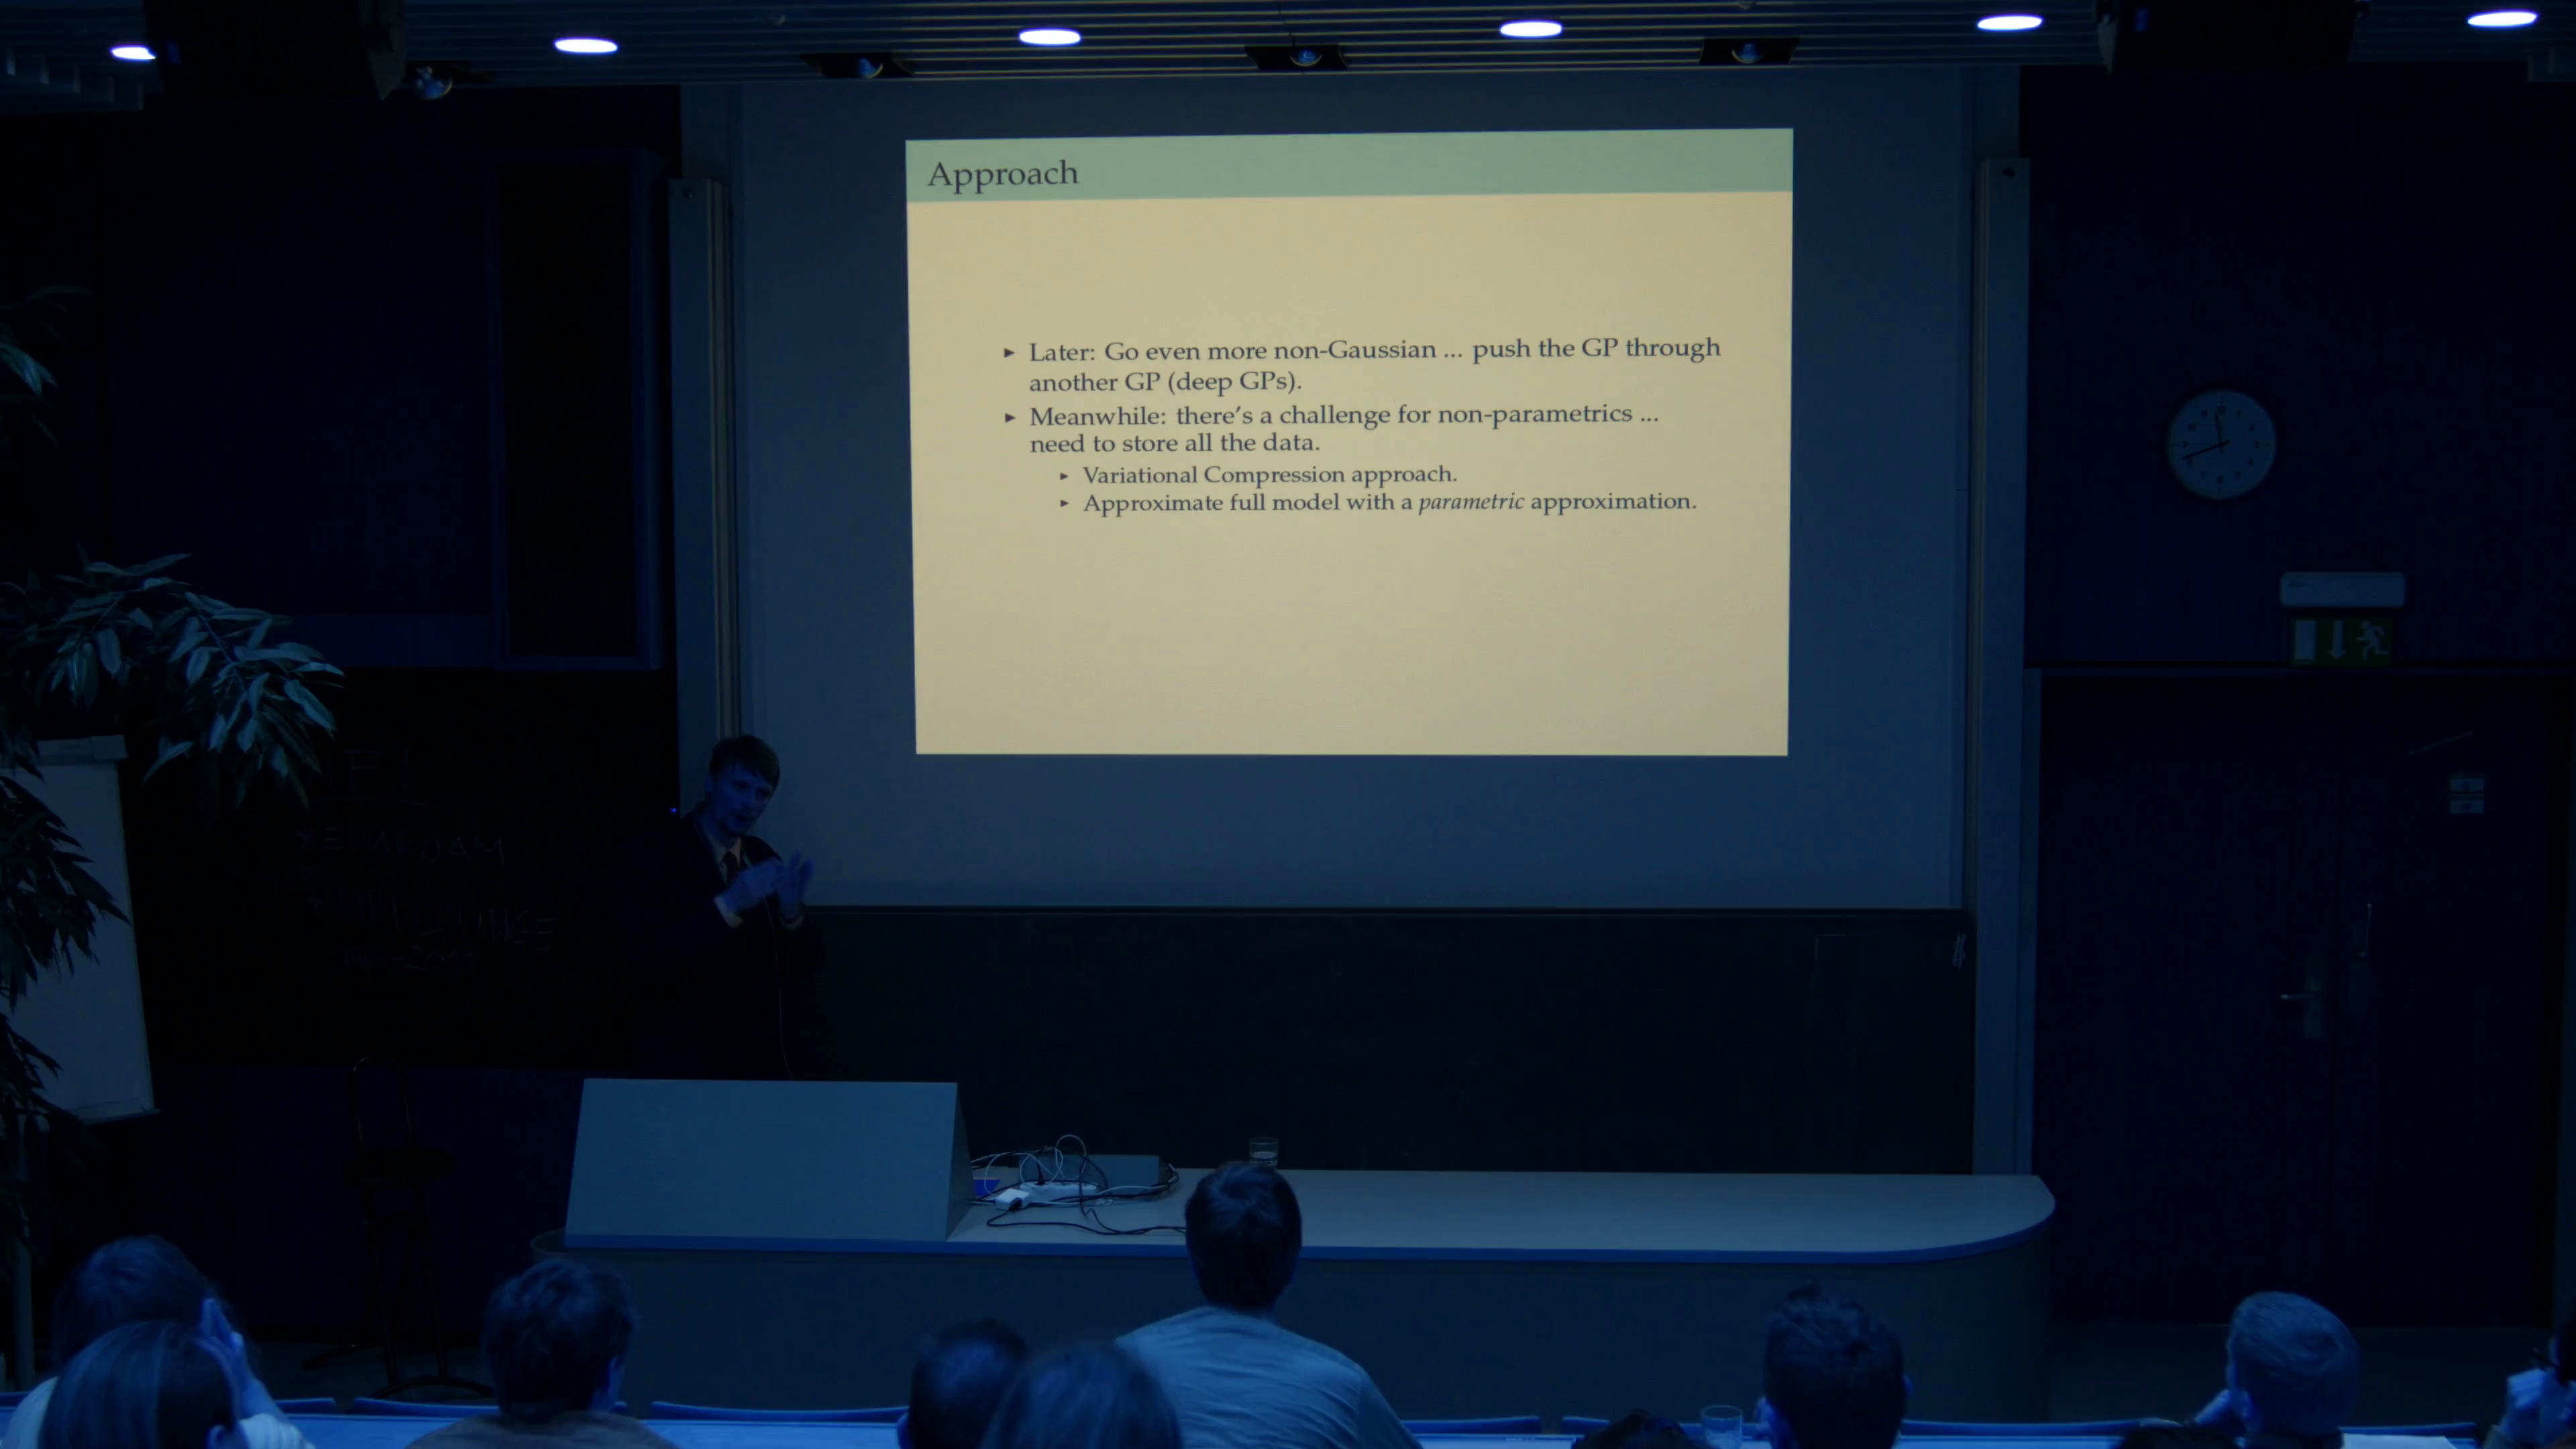
\includegraphics[width=0.15\textwidth]{figures/video.png}};

\node [block, above right =1cm of video]  (vp1) {Pre-Processing};
\node [block, above right  = 0.3cm of vp1]  (vp2) {Slide Detection};
\node [block, below =1.5cm of vp2]  (vp3) {Speaker Tracking};
\node [block, right =3cm of vp1]  (vp4) {Post-Processing};
\node [block, right =1cm of vp4]  (ve5) {Layout Concatenating};
\node [block, right =0.5cm of ve5]  (ve6) {Transcoding/ Filtering};
\node[inner sep=0pt,  below right =1cm of ve6] (layout)  { 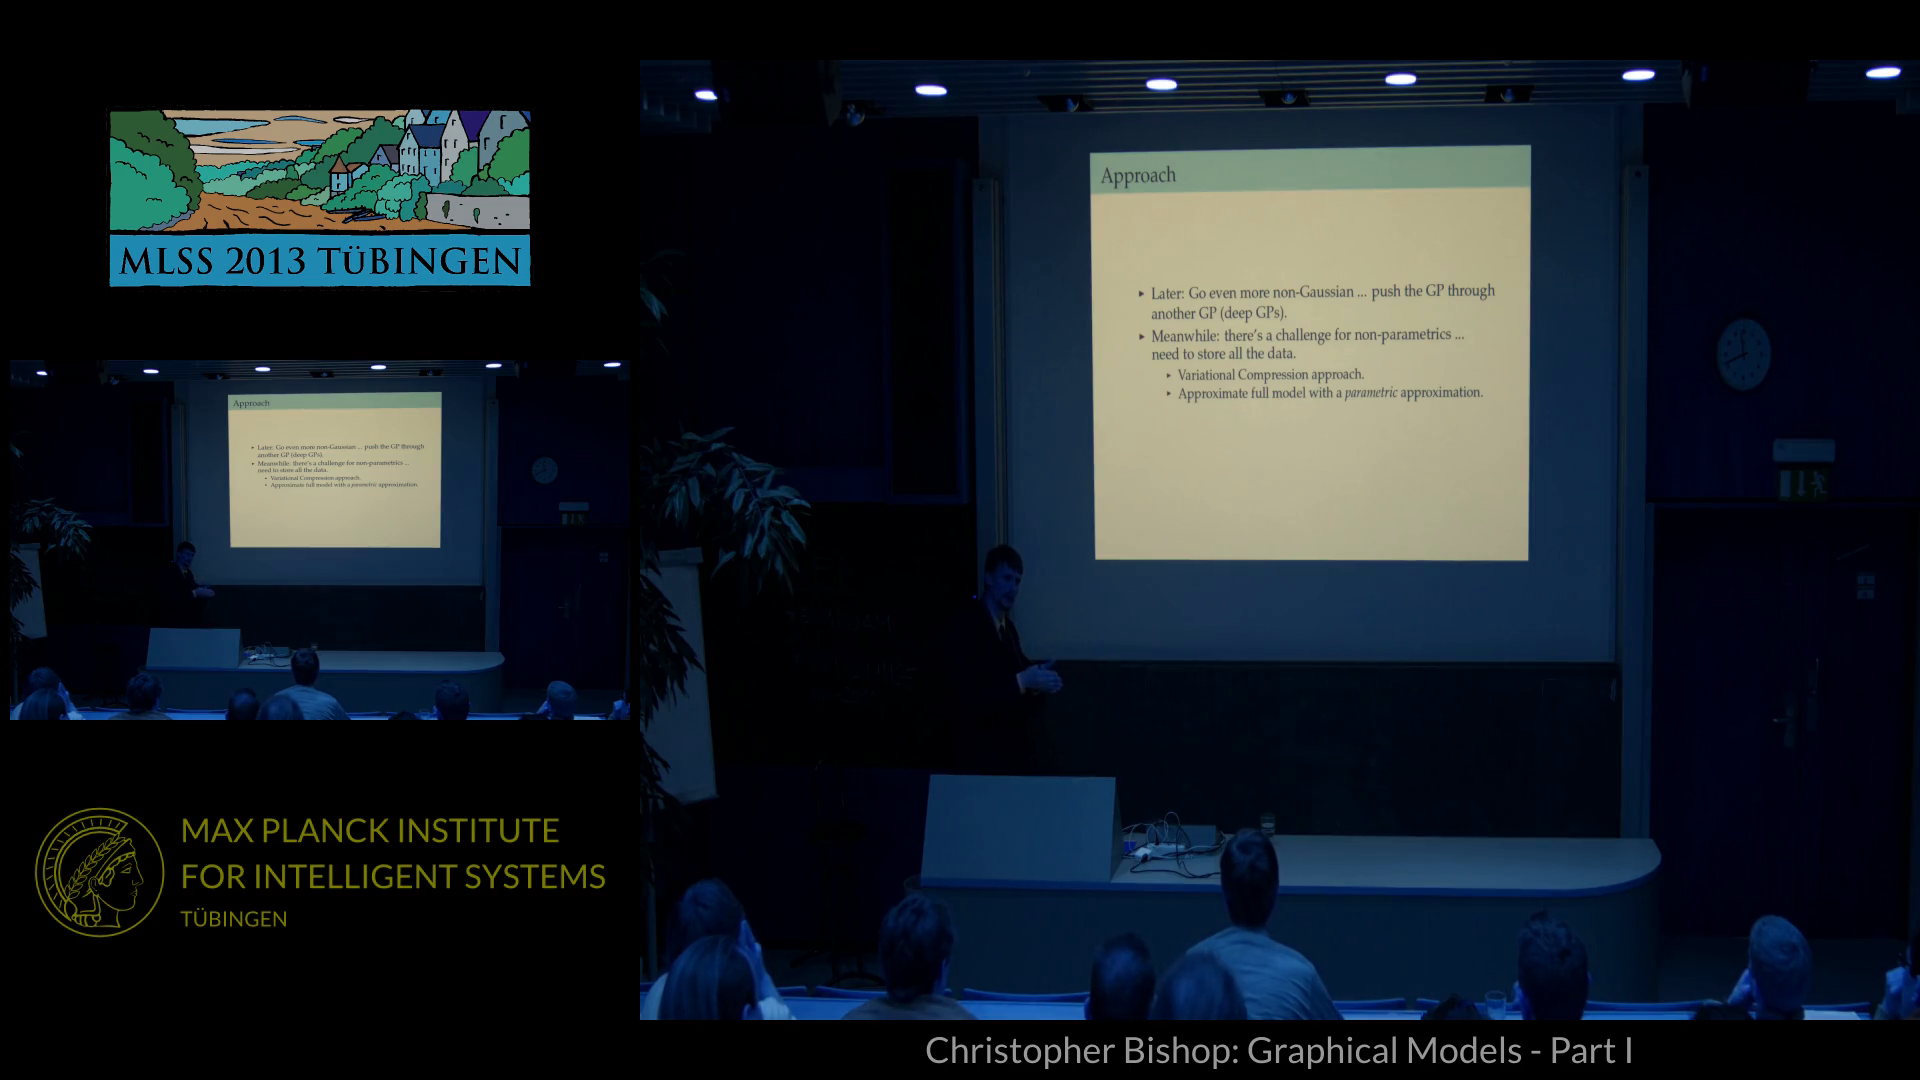
\includegraphics[width=0.15\textwidth]{figures/layout.png}};

\node [block, below right=2.5cm of video]  (ap1) {Equalizer};
\node [block, right=1cm of ap1]  (ap2) {Improvement};
\node [block, right =1cm of ap2]  (ap3) {Transcoding/ Filtering};
\node [block, right =1cm of ap3]  (ap4) {Final Audio file};

\node [ann, below right=1cm of vp4]  (bk) {Background Image};
\node [ann, below =0.01cm of bk]  (info) {Talk/Speaker Info.};

\begin{pgfonlayer}{background}
        \path (vp1.west |- vp2.north)+(-0.3,0.3) node (a) {};
        \path (vp3.south -| vp4.east)+(0.3,-0.3) node (b) {};       
        \path[fill=blue!10,rounded corners, draw=black!50, dashed]
            (a) rectangle (b);           
        \path (vp2.north)+(0.0,+0.5) node (a) {Video Processing};            
 \end{pgfonlayer}


\begin{pgfonlayer}{background}
        \path (ve5.west |- ve5.north)+(-0.3,0.3) node (a) {};
        \path (ve6.south -| ve6.east)+(0.3,-0.3) node (b) {};       
        \path[fill=blue!10,rounded corners, draw=black!50, dashed]
            (a) rectangle (b);           
        \path (ve5.north east)+(0.0,+0.5) node (a) {Video Editing};            
 \end{pgfonlayer}


\begin{pgfonlayer}{background}
        \path (ap1.west |- ap1.north)+(-0.3,0.3) node (a) {};
        \path (ap4.south -| ap4.east)+(0.3,-0.3) node (b) {};       
        \path[fill=blue!10,rounded corners, draw=black!50, dashed]
            (a) rectangle (b);           
        \path (ap2.north east)+(0.0,+0.5) node (a) {Audio Processing};            
 \end{pgfonlayer}



 paths
\path[draw,->] 
          	(vp1) edge (vp2)
          	(vp1) edge (vp3)
	 	(vp3) edge (vp4)
	  	(vp2) edge (vp4)
		(vp4) edge (ve5)
		(ve5) edge (ve6)

	  	(ap1) edge (ap2)
		(ap2) edge (ap3)
		(ap3) edge (ap4)
;
               
\draw[-latex] +(1,1.5) node (a) {Video}(video.east) -- ++(0.5,0)  |-  (vp1.west) ;
\draw[-latex] +(1,-1.5) node (a2) {Audio}(video.east) -- ++(0.5,0) |-  (ap1.west);

\draw[-latex] (ve6.east) -- ++(0.5,0) |-  (layout.west);
\draw[-latex] (ap4.east) -- ++(0.95,0) |-  (layout.west);

\draw[-latex] (bk.west) -- ++ (-0.2,0.0) |-  (ve5.west);
\draw[-latex] (info.west) -- ++(-0.2,0.0) |-  (ve5.west);


\end{tikzpicture}
}
\vspace{-0.3cm}
    \caption{\small The whole framework}
    \label{fig_framework}
\centering
\end{figure}




\begin{figure}[ht]
	\centering

	\begin{subfigure}[b]{0.30\textwidth}
	\resizebox{1\linewidth}{!}{
\pgfdeclarelayer{background}
\pgfdeclarelayer{foreground}
\pgfsetlayers{background,main,foreground}

\begin{tikzpicture}[>=latex']

\draw (0,0)  node[xshift=-0.5cm,yshift= 2cm, text width=0.5cm, black ,font=\small]{1320} -- (6,0) -- (6,4) -- (0,4)  node[xshift=4.2cm,yshift= 0.2cm, text width=3cm, black ,font=\small]{1920} -- (0,0);
\draw[thick,-] (2,0) -- (2,4);
\draw[thick,-] (0,1.33)  -- (2,1.33) node[xshift=-1cm,yshift= 0.7cm, text width=1cm, black ,font=\small]{Speaker 640x360};
\draw[thick,-] (0,2.66) -- (2,2.66);
\draw[thick,-] (2,0.5) -- (6,0.5)  node[xshift=-2cm,yshift= 1.5cm, text width=1cm, black ,font=\small]{Slide 1280x960};
\draw[thick,-] (2,3.5) -- (6,3.5);

\end{tikzpicture}
}
	      \caption{\small Video layout}
		\label{fig_layout_a}
	\end{subfigure} 
	\begin{subfigure}[b]{0.30\textwidth}
	      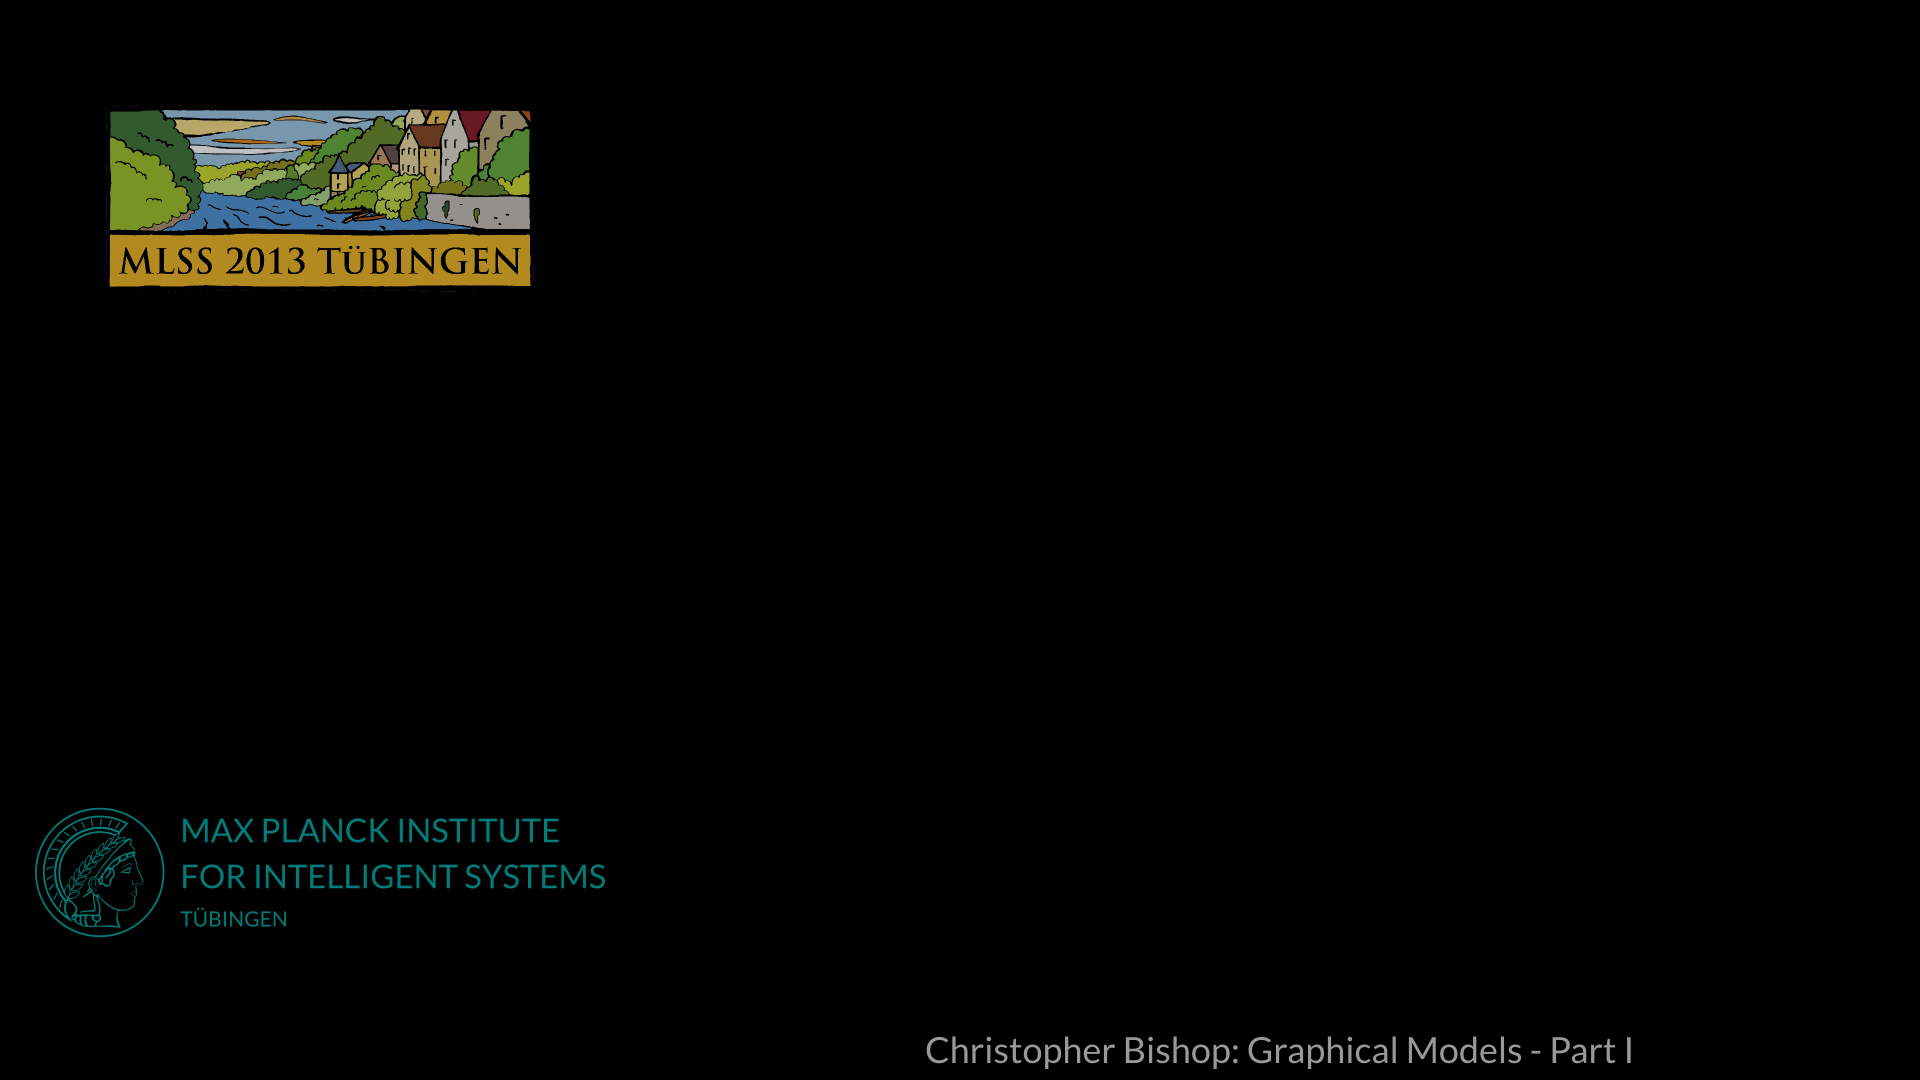
\includegraphics[width=\textwidth]{figures/background_example.png}
	      \caption{\small Background image}
		\label{fig_layout_b}
	\end{subfigure}	       
	\begin{subfigure}[b]{0.30\textwidth}
	       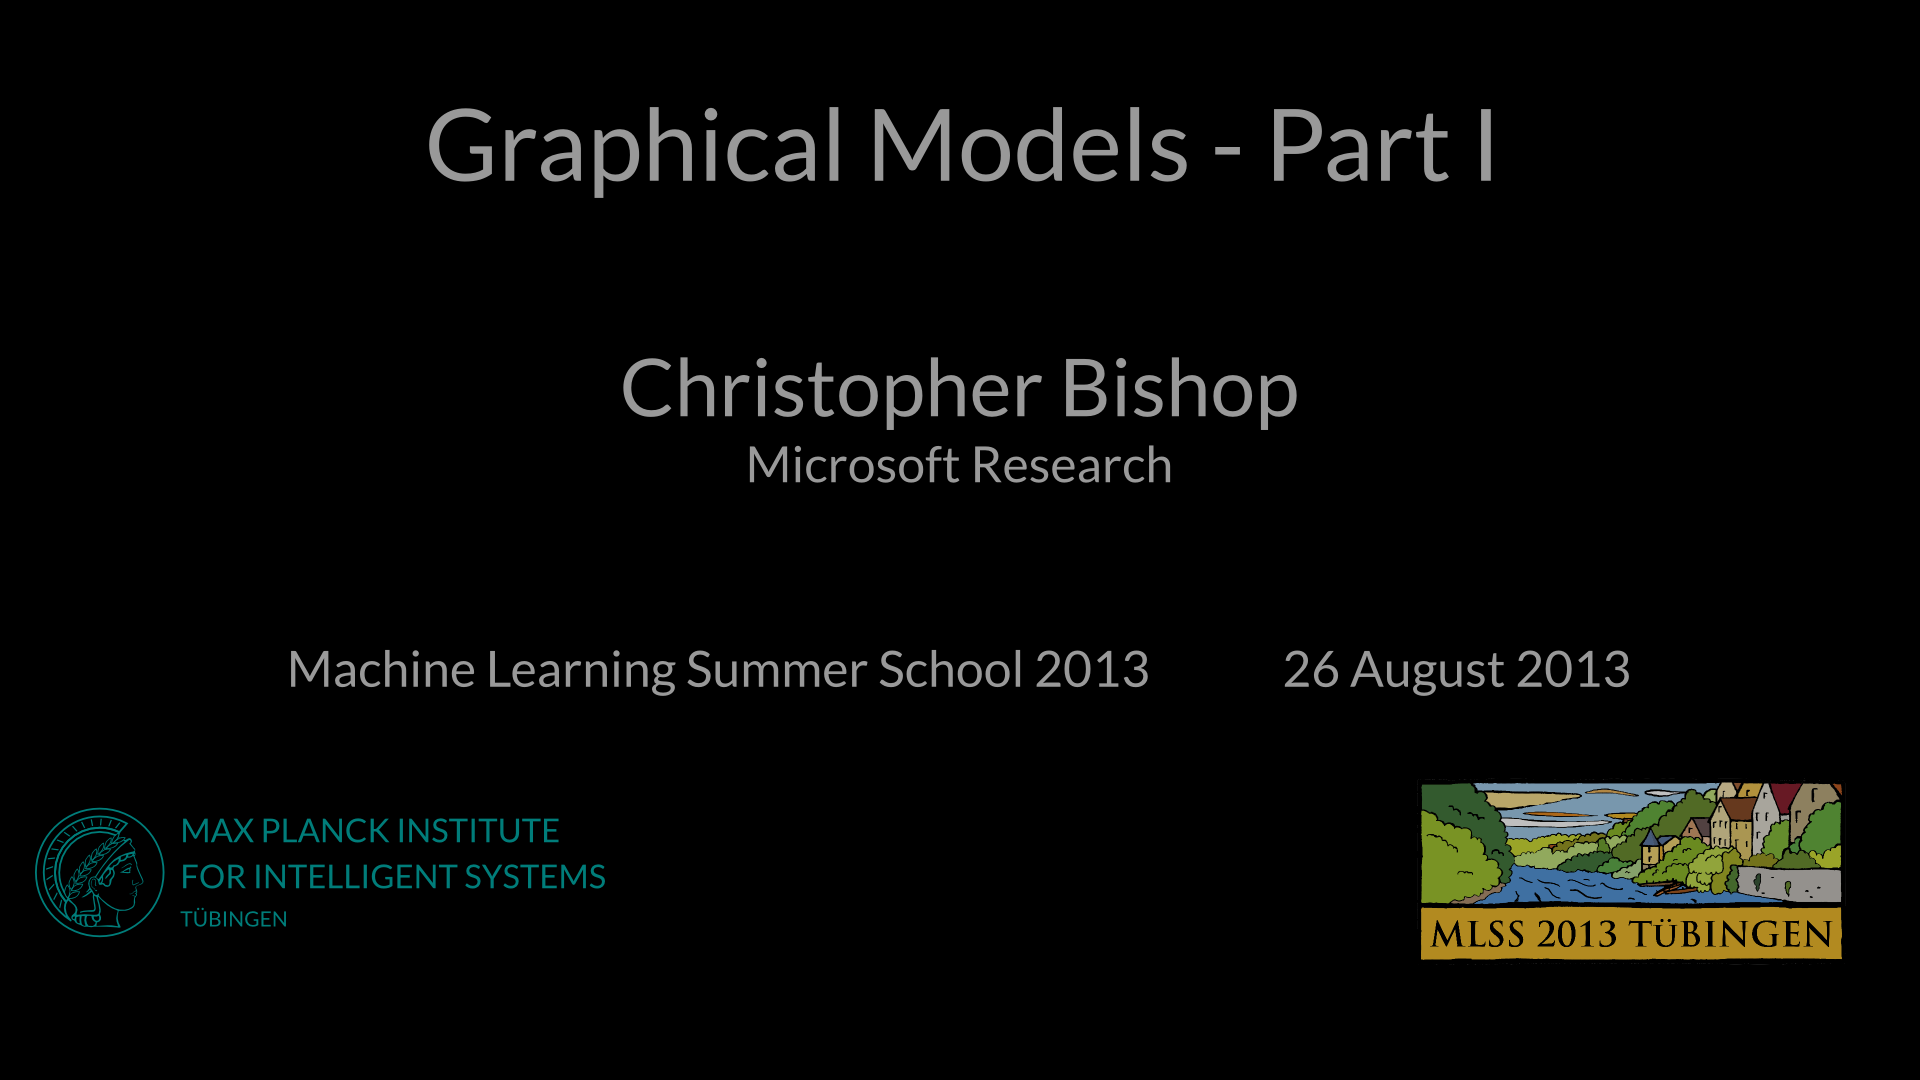
\includegraphics[width=\textwidth]{figures/title_example.png}
	       \caption{\small First Info. slide}
	\label{fig_layout_c}
	\end{subfigure}
	\caption{The final video layout}
	\label{fig_layout}
\end{figure}







\section{Requirements}




\subsection{Hardware}

The current hardware and tools are shown in figure \ref{fig_hw}. 
Figure \ref{fig_hw_b} indicates the 4-TB SSD hard along with the corresponding docking station. There are 4 SSDs, totally 16 TB. These Hard drives should be used for the backup of raw videos. 
Figure \ref{fig_hw_c} is the 2-TB USB3.0 external hard disk for any mobility.  
Figure \ref{fig_hw_d} shows the 1-TB Solid State Drive (SSD) which suits with Blackmagic camera. There should exist two of them.
Fig \ref{fig_hw_e} includes Sata HDD docking station and reader along with its secondary power supply and USB3.0 port. 
Figure \ref{fig_hw_f} indicates the 4k Blackmagic Camera, its power supply, audio cables and the ultrasonic 24mm lens. 
Besides the shown laptop, there is another desktop PC as an implementation platform with following properties.

\begin{itemize}
	\item Processor: Intel® Core™ i7-5930K CPU @ 3.50GHz × 12 
	\item Memory: 32 GiB
	\item Graphic: NVIDIA GeForce GTX 750/PCIe/SSE2
	\item Disk: 3 Data raid for 12 TB
	\item Operating system: Ubuntu 14.04 and windows 7
\end{itemize}


\begin{figure}[ht]
	\centering
	\begin{subfigure}[b]{0.29\textwidth}
	       \includegraphics[width=\textwidth]{figures/1_(1).png}
	       \caption{}
		\label{fig_hw_a}
	\end{subfigure} 
	\begin{subfigure}[b]{0.30\textwidth}
	      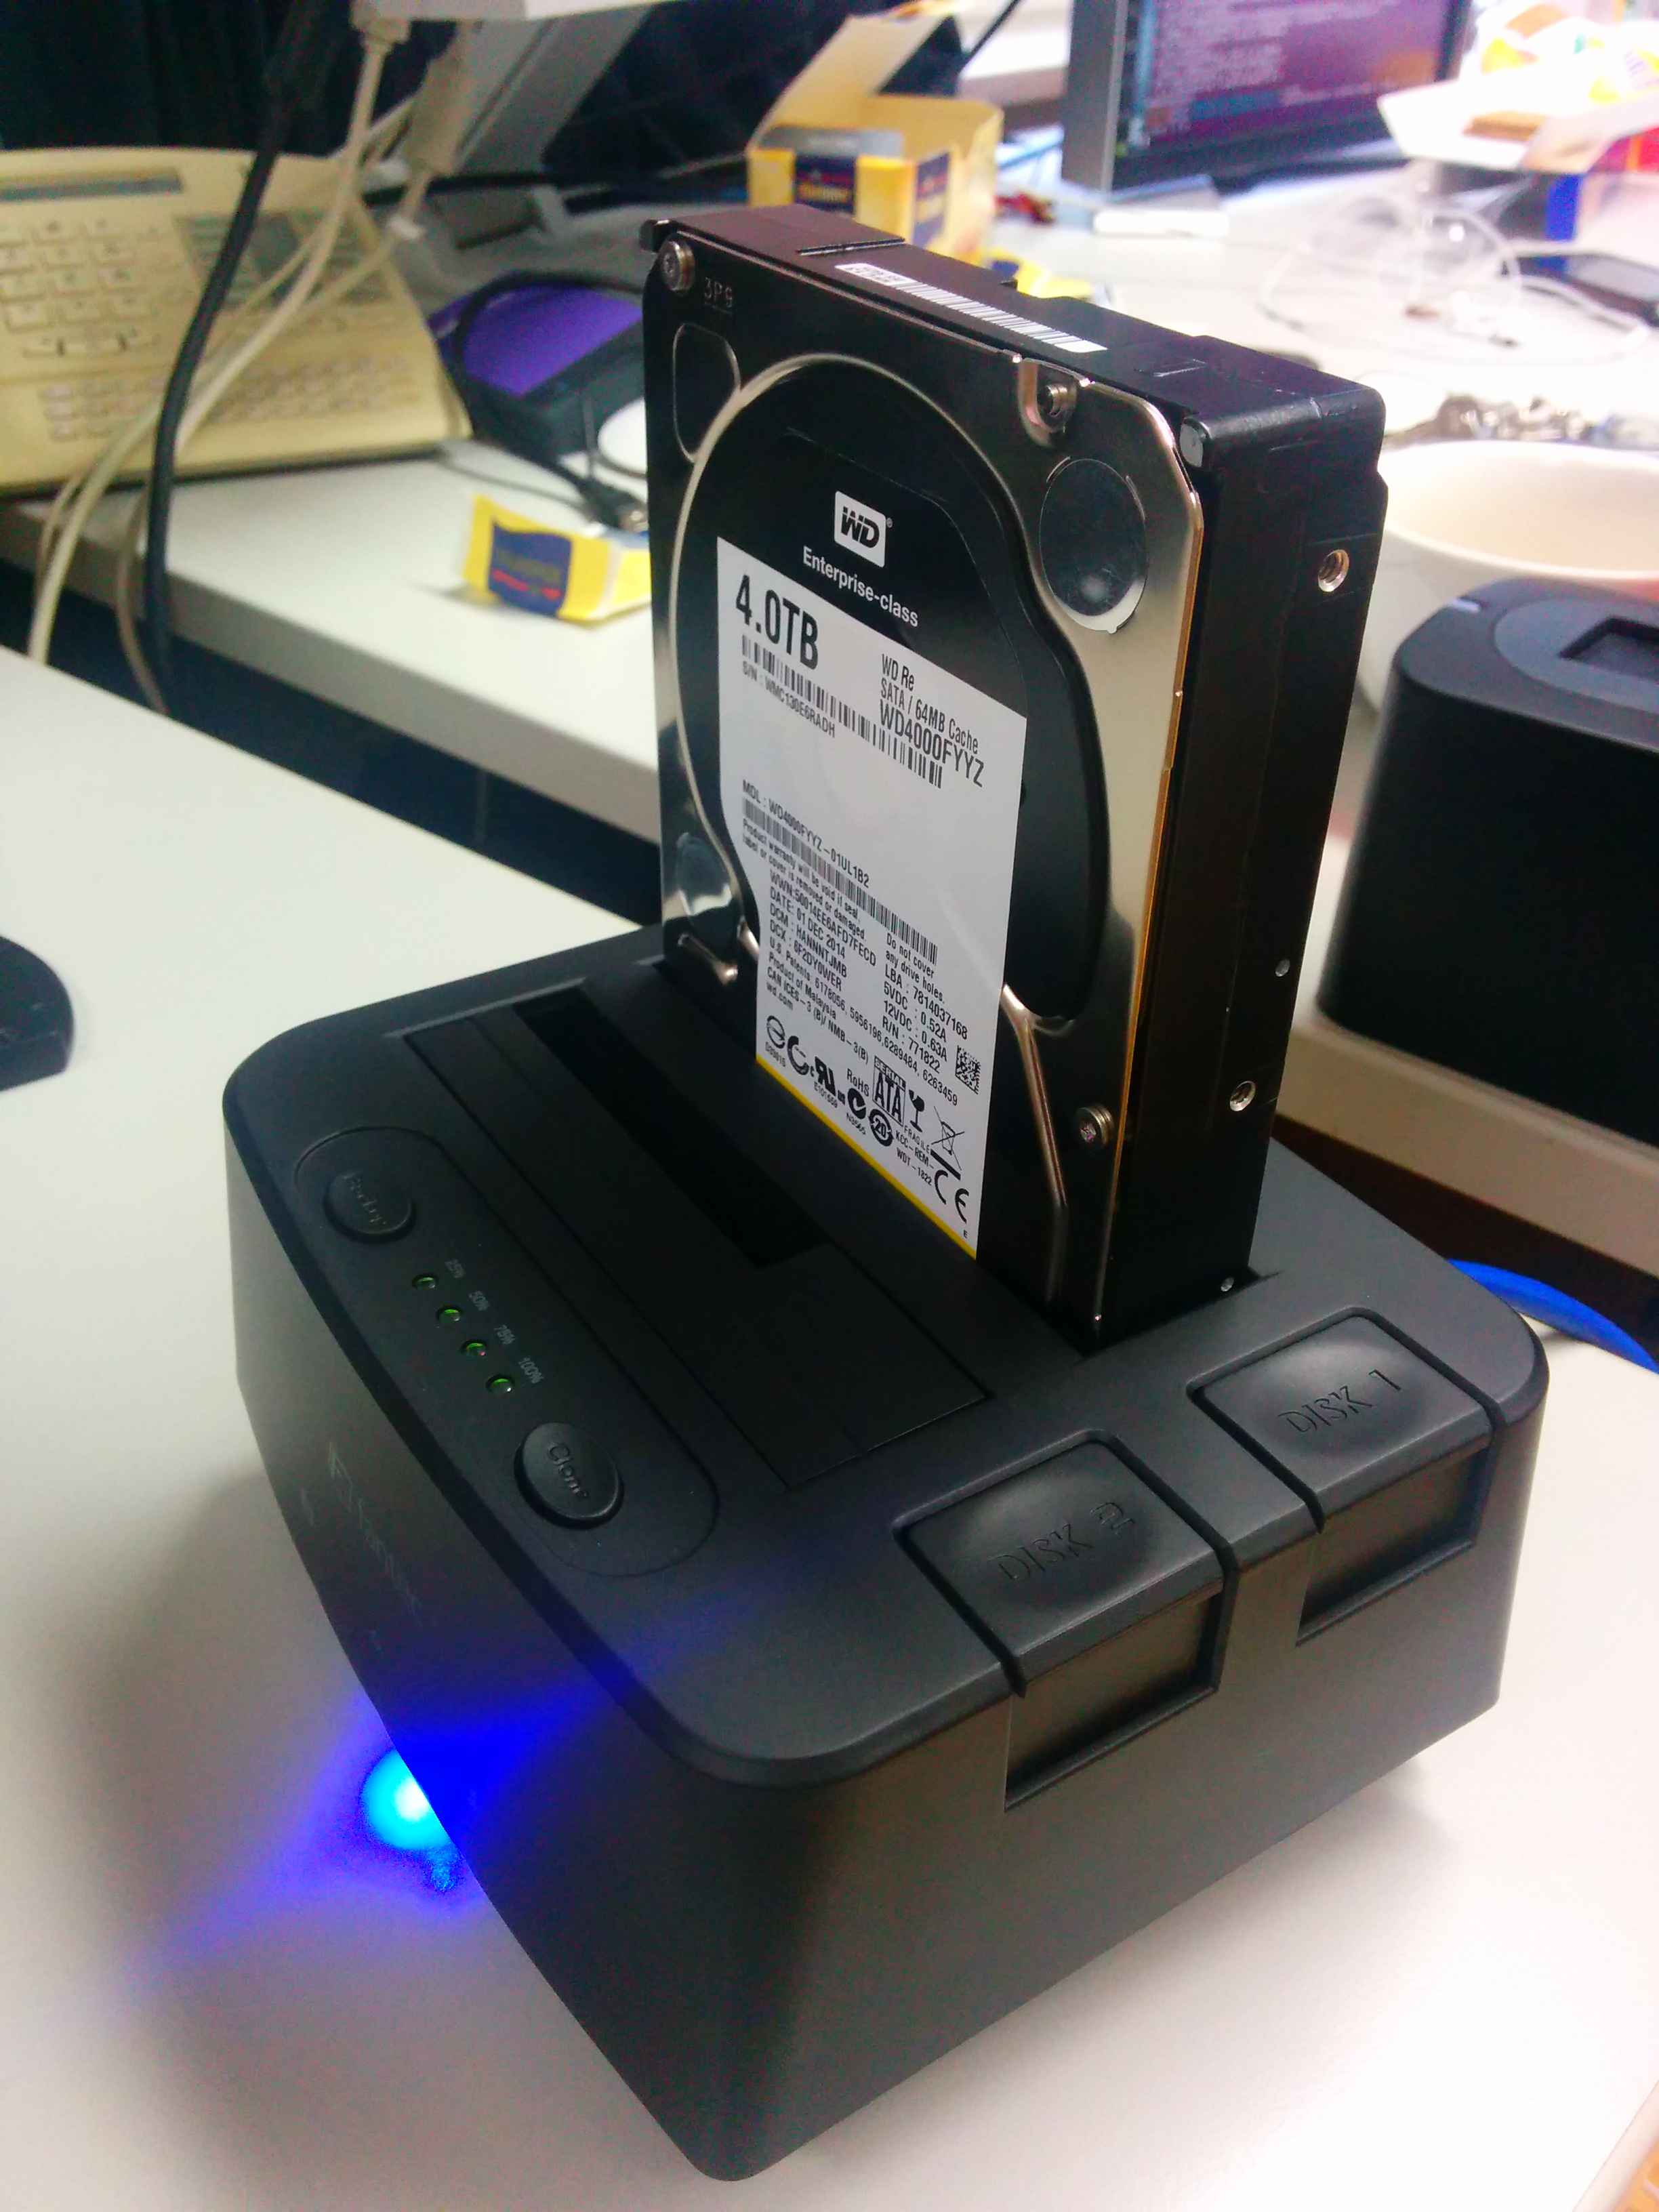
\includegraphics[width=\textwidth]{figures/n1.jpg}
	      \caption{}
		\label{fig_hw_b}
	\end{subfigure}	        
	\begin{subfigure}[b]{0.30\textwidth}
	       \includegraphics[width=\textwidth]{figures/1_(3).png}
	       \caption{}
	\label{fig_hw_c}
	\end{subfigure}

	\begin{subfigure}[b]{0.30\textwidth}
	      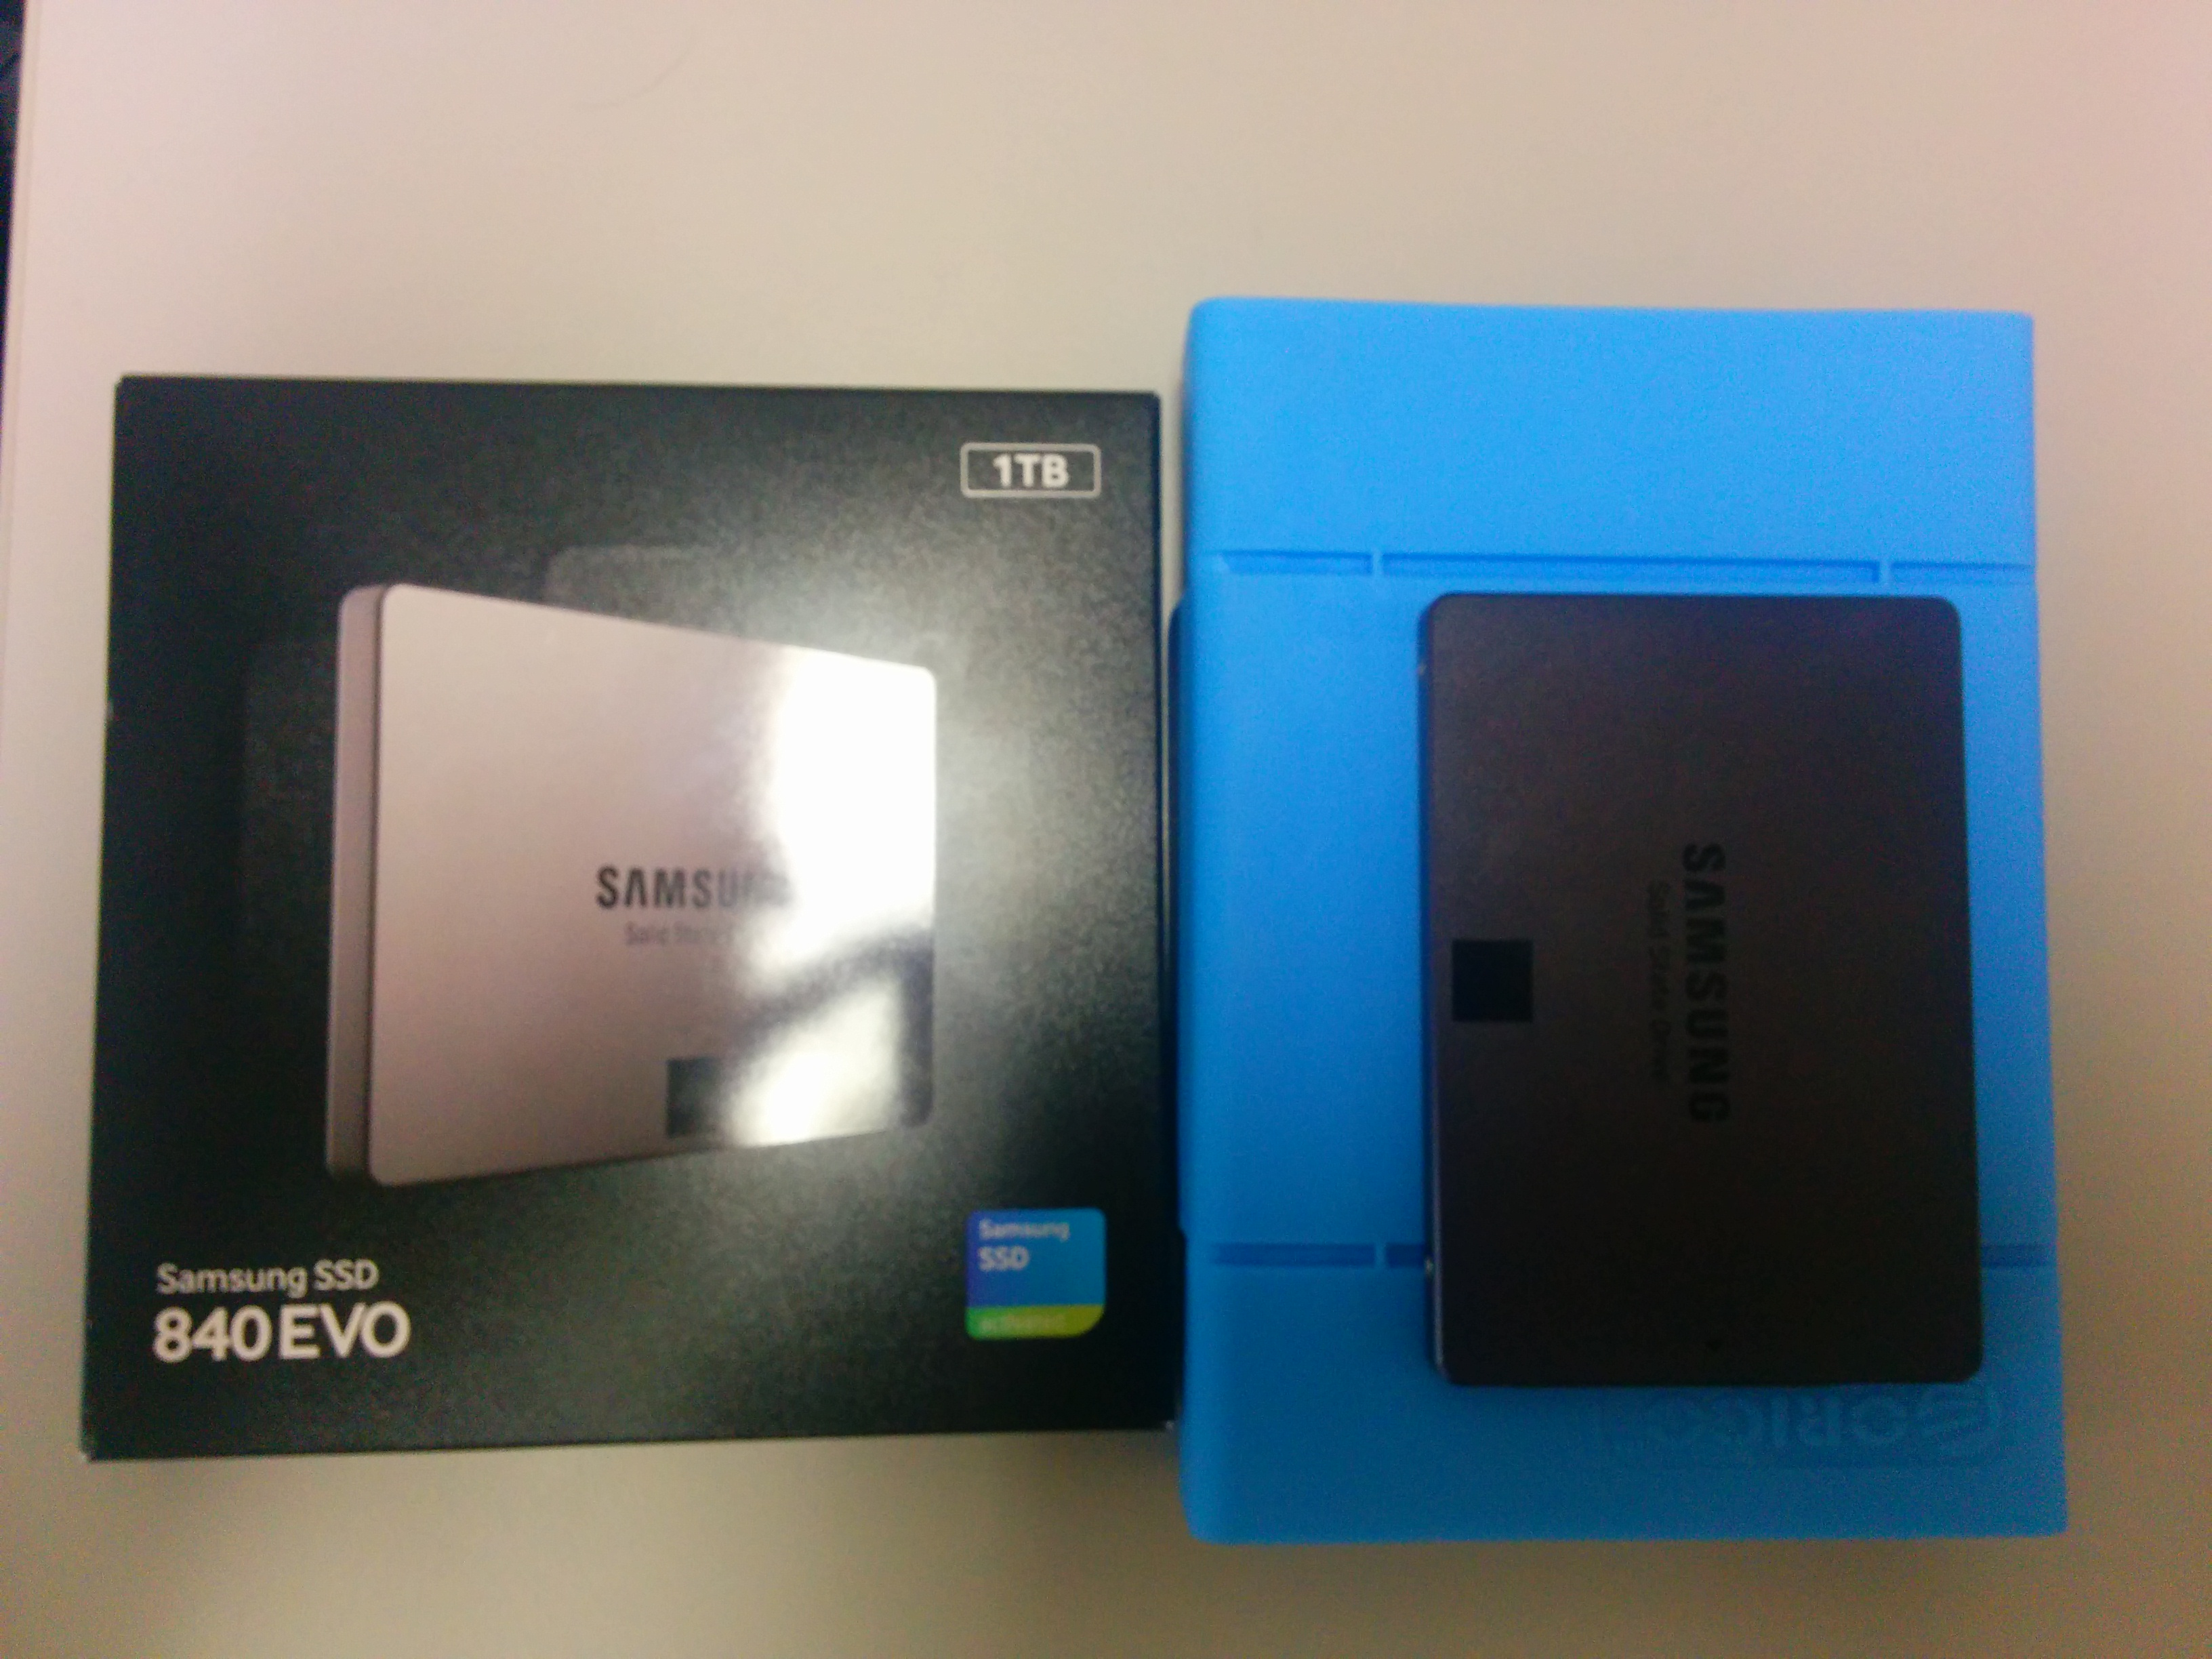
\includegraphics[width=\textwidth]{figures/n3.jpg}
	      \caption{}
		\label{fig_hw_d}
	\end{subfigure}
	\begin{subfigure}[b]{0.30\textwidth}
	      \includegraphics[width=\textwidth]{figures/1_(4).png}
	      \caption{}
		\label{fig_hw_e}
	\end{subfigure}
	\begin{subfigure}[b]{0.30\textwidth}
	      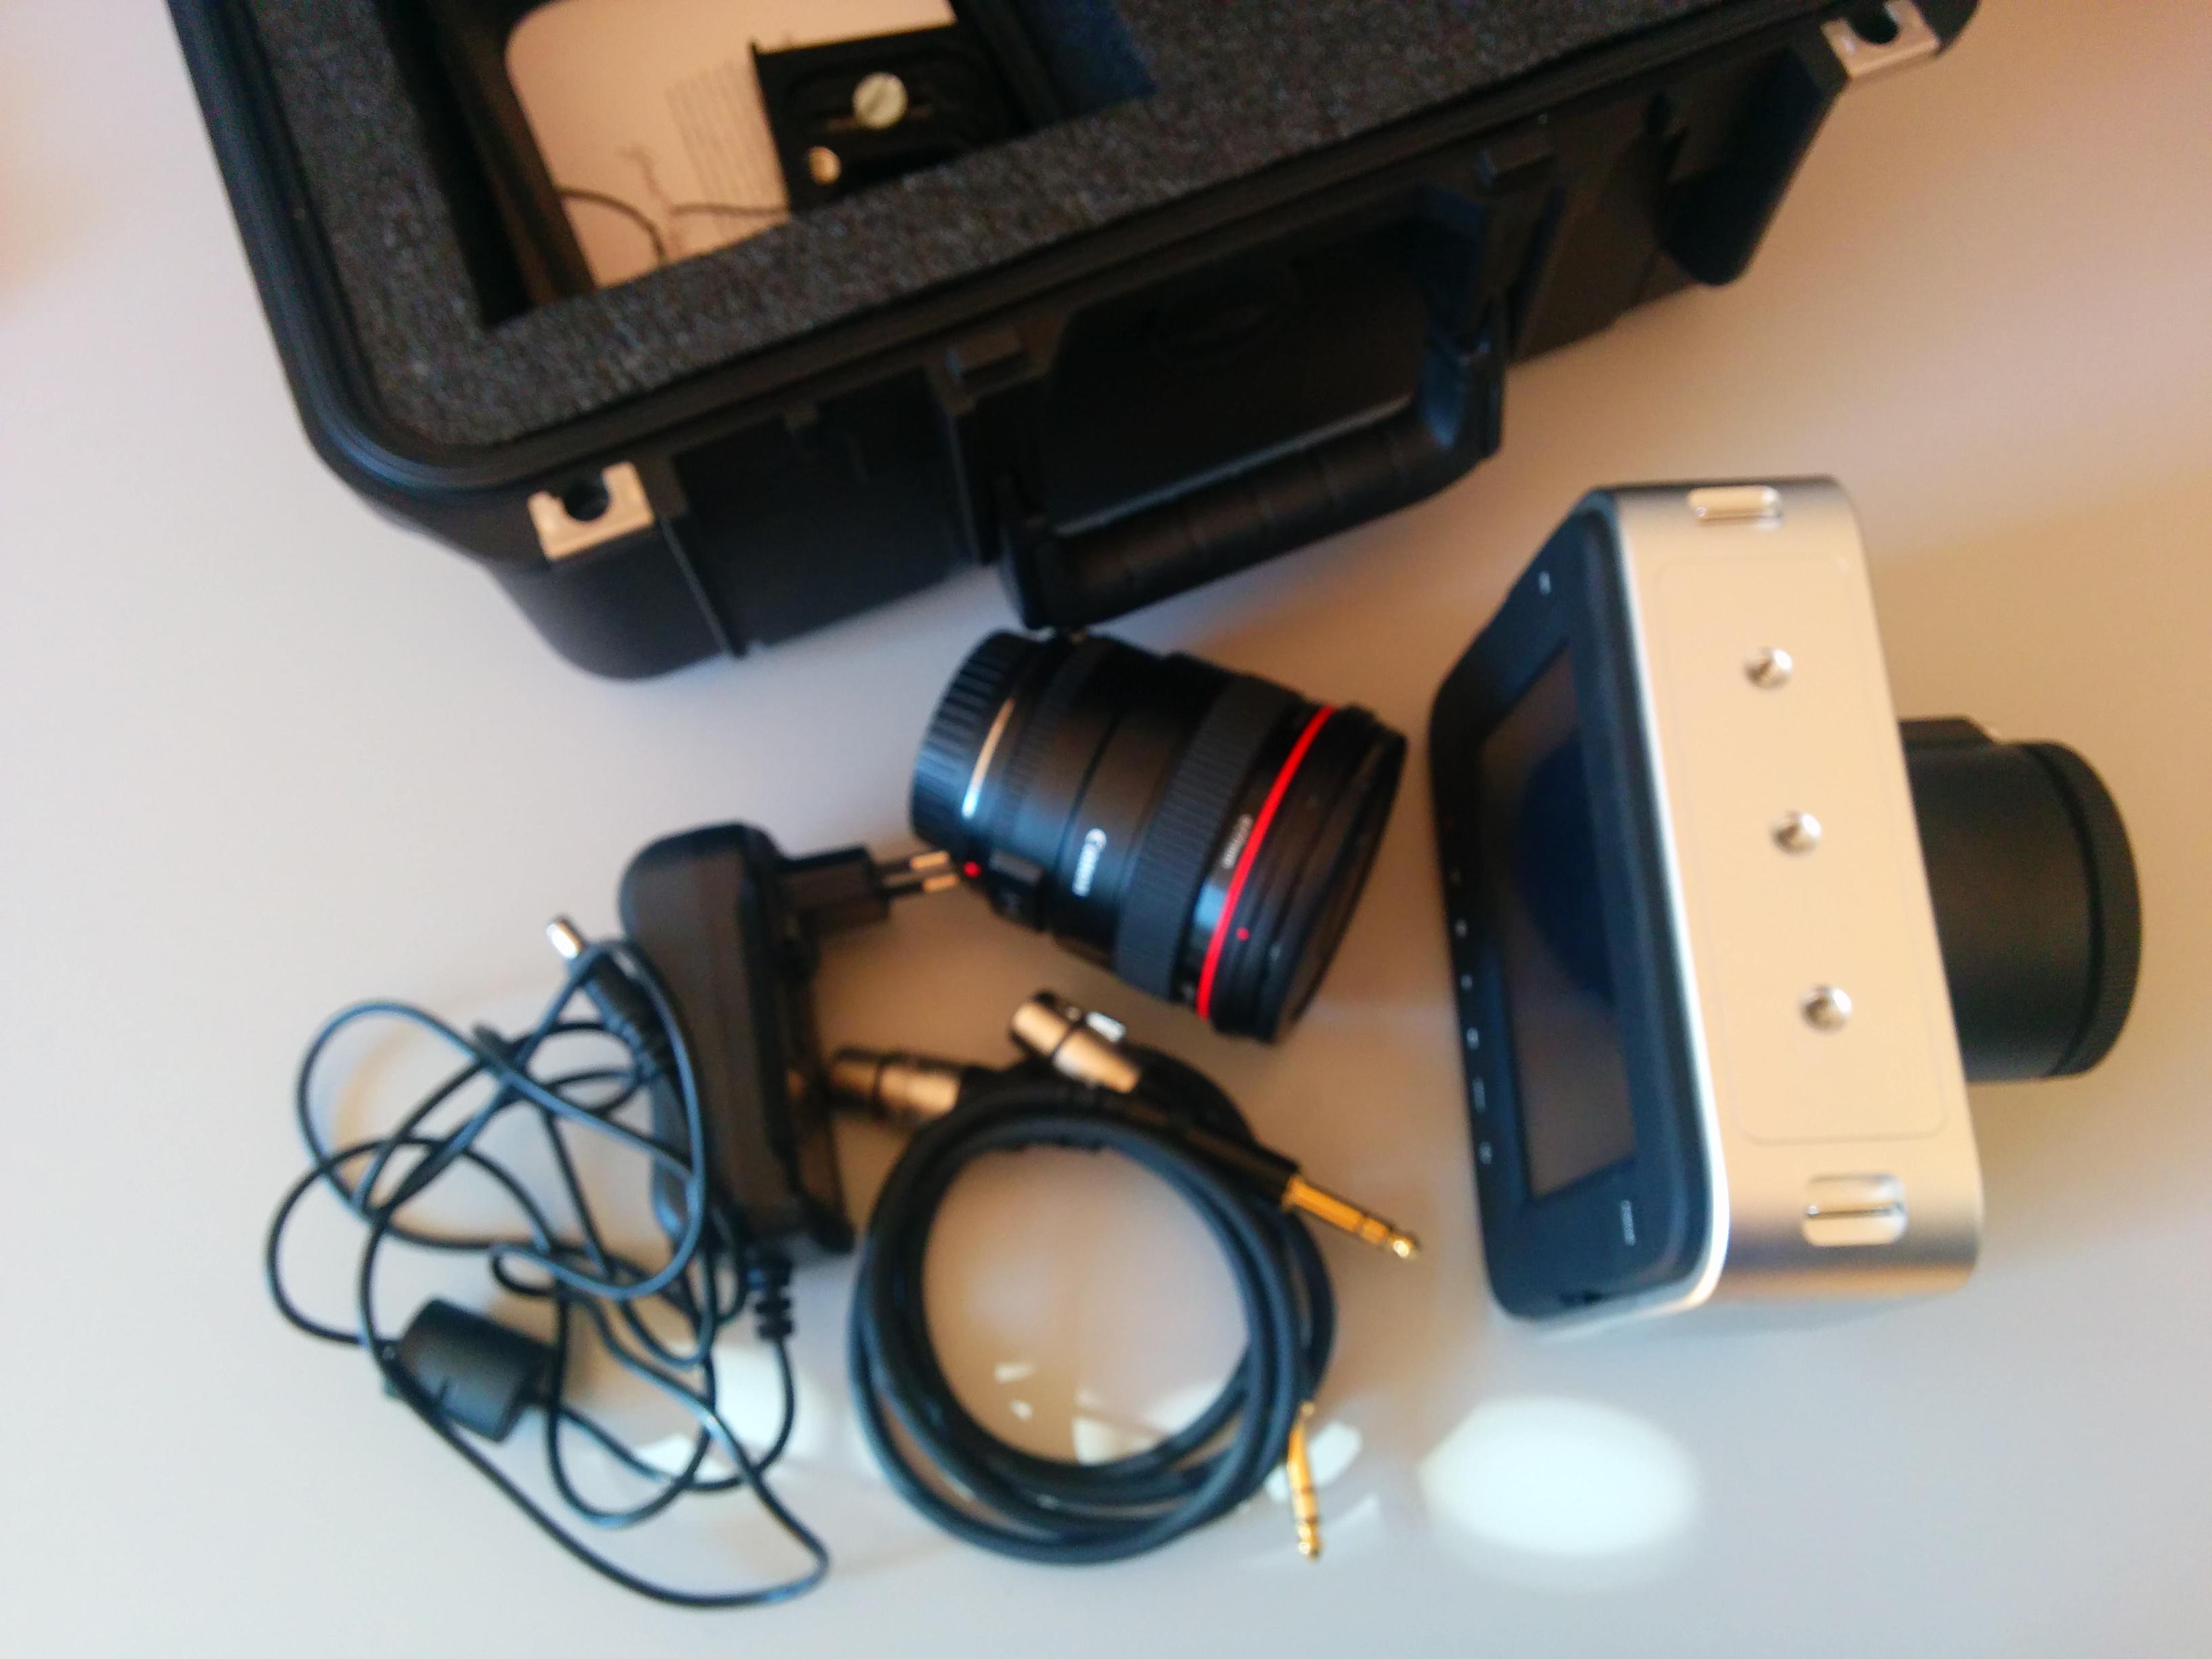
\includegraphics[width=\textwidth]{figures/1_(2).jpg}
	      \caption{}
		\label{fig_hw_f}
	\end{subfigure}
	\caption{The hardwares}
	\label{fig_hw}
\end{figure}



\subsection{Software}

There are two major aspects which should be taken into account in this work. As it was already mentioned the framework needs both video processing and video editing. Since, there is no open source library to handle both tasks, It is better to stay with C++ or Python. To this end, we checked several libraries and tools listed as follow.

\begin{enumerate}
\item Nuke production:

A software for composing multiple images and effects, motion graphics, not open source, no good documentations. It seems to be for design, film editing, visualization, etc. \url{https://www.thefoundry.co.uk/products/nuke/}

\item MLT framework:

It is an open source tool based on C++ for audio/video editing, media trasncoding, web stream and TV broadcasting. \url{http://www.mltframework.org/}


\item MoviePy:

MoviePy is a Python module for video editing, which can be used for basic operations (like cuts, concatenations, title insertions), video compositing, or to create advanced effects. It can read and write the most common video formats. \url{http://zulko.github.io/moviepy/}

\end{enumerate}

In order to develop new algorithms as convenient as possible, it was decided to take advantages from pre-built libraries and use Python language ( Python 2.7.6 where /usr/bin/python). The major required libraries and packages have been listed as below.



\begin{itemize}
	\item Moviepy
	\item ffmpeg
	\item OpenCV-2.4.8	
\end{itemize}



\subsubsection{Software Installation}

In order to get Livius framework running  on your local machine/laptop, one can easily follow the guided installation depicted in this section. The instruction is under linux operating system and it has tested on Ubuntu 14.04.

\paragraph{Python}

The first assumption to run the system is to have python installed on your local machine. You may find different Python versions   released in the \url{https://www.python.org/downloads/} \cite{python}. To check whether you have already installed the python or not and find the version, you can use the command \texttt{which python} and \texttt{python --version} in terminal. If you do not have it, then firstly you need to install some dependencies, therefore:

\begin{framed}
 
(sudo) apt-get install build-essential

(sudo) apt-get install libreadline-gplv2-dev libncursesw5-dev libssl-dev libsqlite3-dev tk-dev libgdbm-dev libc6-dev libbz2-dev

\end{framed}


Then download using the following command, extract the files and go to the directory

\begin{framed}

cd \char`\~/Downloads/

wget http://python.org/ftp/python/2.7.6/Python-2.7.6.tgz

tar -xvf Python-2.7.6.tgz

cd Python-2.7.6

\end{framed}

Now, install using the command as below:

\begin{framed}

./configure

make

sudo make install

\end{framed}


After installing the python, you can simply type \texttt{python} for python prompt. The next step is to install your required python packages. It is strongly recommended to install \lq\lq pip\rq\rq which is a package management system used to install and manage packages written in Python. \lq\lq pip\rq\rq should be included for Python 2.7.9 and later (on the python2 series), and Python 3.4 and later by default. (You may us get-apt package manager as well.)

\begin{framed}

sudo apt-get update

sudo apt-get install python-pip

\end{framed}

you have to install the listed python packages.


\begin{framed}

sudo apt-get install python-pygame

sudo apt-get install python-matplotlib 

sudo apt-get install python-scipy

sudo apt-get install python-numpy


\end{framed}

\paragraph{Moviepy}

As it was mentioned, \lq\lq moviepy\rq\rq is one of the requirements to get the framework running as we use many methods from that \cite{moviepy} .
MoviePy depends on the Python modules Numpy, imageio, Decorator, and tqdm, which will be automatically installed during MoviePy's installation. 

\begin{framed}

(sudo) pip install moviepy

\end{framed}


\paragraph{ffmpeg}

In order to install \lq\lq ffmpeg\rq\rq on your local computer, please follow the instruction on the website \url{https://trac.ffmpeg.org/wiki/CompilationGuide/Ubuntu}.


\paragraph{OpenCV}

To run the OpenCV's libraries, one needs the cmake 2.8.12.2. Therefore, it does not exist on your O.S., use the following command.

 \begin{framed}

sudo apt-get install cmake

\end{framed} 


 If you are running 13.10 and you don't have a nvidia card then ensure you install \lq\lq ocl-icd-libopencl1\rq\rq. Ubuntu 13.10 will install nvidia-319-updates as a dependency for libopencv-dev by default if ocl-icd-libopencl1 is not installed.

 \begin{framed}

sudo apt-get install ocl-icd-libopencl1

\end{framed} 


To Install OpenCV on Ubuntu or Debian, you can do it from the repository or manually. a very good tutorial for this purpose is addressed in \url{http://milq.github.io/install-opencv-ubuntu-debian/}. You can install OpenCV from the repository.

 \begin{framed}

sudo apt-get install libopencv-dev python-opencv

\end{framed} 

However, you will probably not have installed the latest version of OpenCV and you may miss some features (for example: Python 3 bindings do not exist in the repository). Therefore, install it manually with the help of mentioned link.

\paragraph{pykalman}

pykalman depends on the following modules,


\begin{itemize}

\item numpy (for core functionality)
\item scipy (for core functionality)
\item Sphinx (for generating documentation)
\item numpydoc (for generating documentation)
\item nose (for running tests)

\end{itemize}

All of these and pykalman can be installed using \texttt{easy\_install}  as:

 \begin{framed}

\texttt{easy\_install} numpy scipy Sphinx numpydoc nose pykalman

\end{framed} 

Alternatively, you can get the latest and greatest from github like 

 \begin{framed}

git clone git@github.com:pykalman/pykalman.git pykalman

cd pykalman

 sudo python setup.py install

\end{framed} 

The installation instruction can be found in \url{https://github.com/pykalman/pykalman}.


\section{Initial Attempts}

\subsection{Camera Setting}

4k Blackmagic camera has different coding formats to store the recorded data and it supports two full HD sizes such as 4k and 2k videos . The 2k has 1920x1080 pixels while the size of the 4k video recording is 3840x2160. For each one, there are four different codecs. The codecs are ProRes Proxy, ProRes LT, ProRes 422 and ProRes HQ so that the first one has the lowest quality and the last one takes the highest. Figure \ref{fig_cam} shows the main menu and the sub-menus of the 4k blackmagic camera. This camera has two  disk formats like HFS+ and exFAT (Figure \ref{fig_cam_b}). The former supports Mac OS and the latter works for windows. There in no format for Linux. The most important part of the menu is setting by which one is able to specify various adjustments. The setting part has 4 different sections.  

\begin{enumerate}

	\item Camera (figure \ref{fig_cam_c})

	Here, it is possible to adjust camera Id, date, time, ISO, white balance and shutter angle. In our records, the ISO, white balance and shutter angle have been adjusted into 400, 5200k and 180$^{\circ}$ respectively.

	\item Audio (figure \ref{fig_cam_d})

	The second section is related to audio adjustments and two microphones inputs.

	\item Recording (figure \ref{fig_cam_e})

	The third part supports the recording task and provides different options. In recording format, one can choose either the raw data or one of the 8 codecs. Here, one might determine the fps and time lapse. In our experiments, we use 30 fps.	

	\item Display

	It includes some adjustments corresponding to the screen display of camera like brightness and so on.


\end{enumerate}



\begin{figure}[ht]
	\centering
	\begin{subfigure}[b]{0.30\textwidth}
	       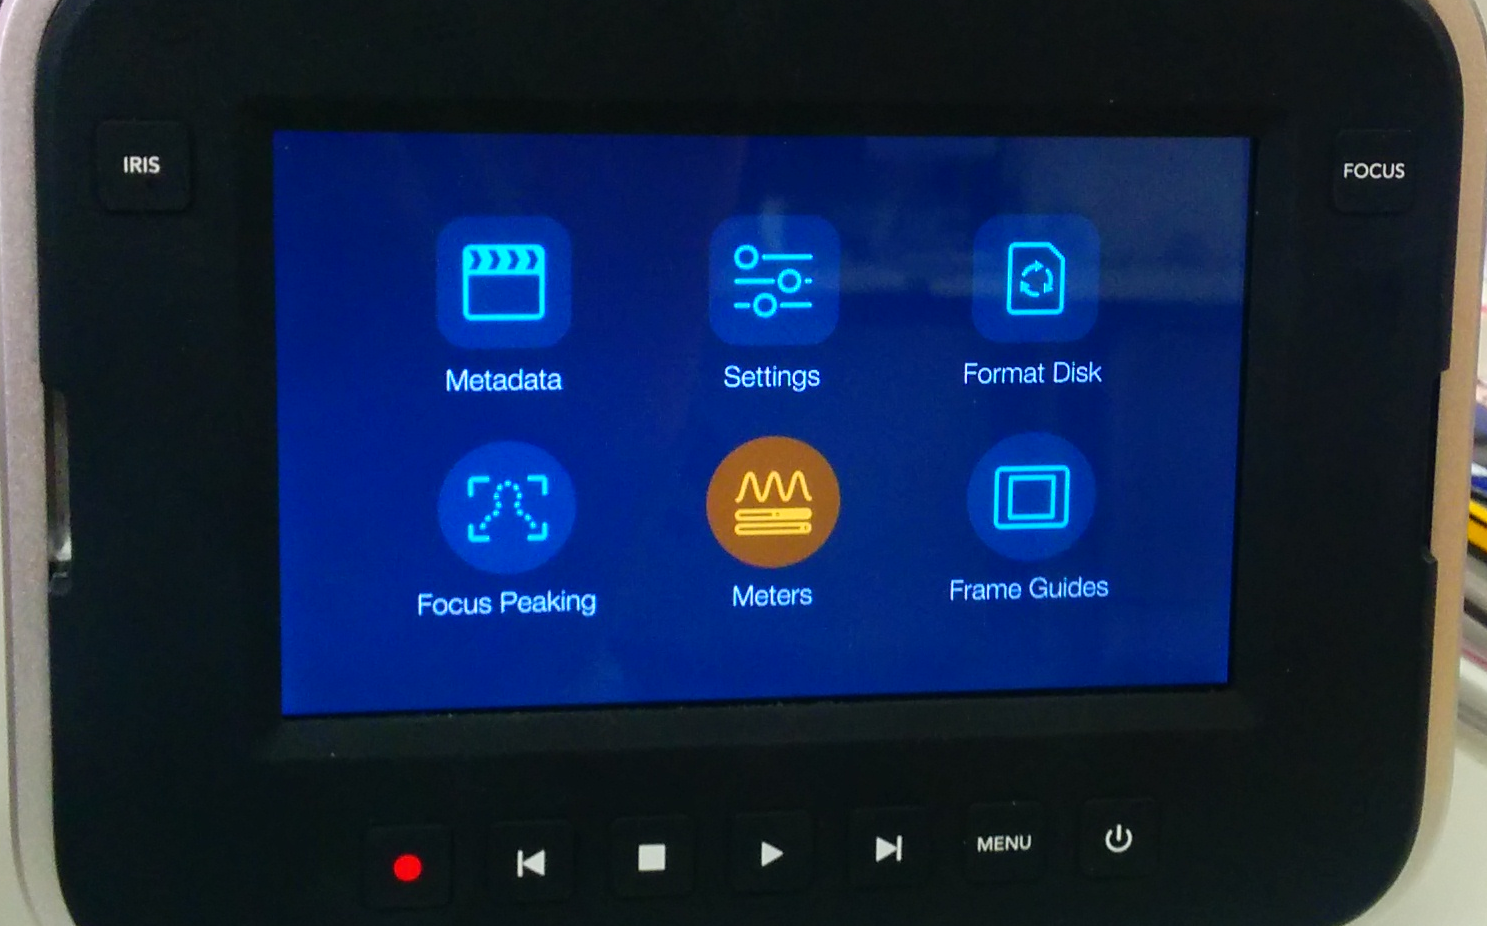
\includegraphics[width=\textwidth]{figures/camera2.png}
	       \caption{The main menu}
		\label{fig_cam_a}
	\end{subfigure} 

	\begin{subfigure}[b]{0.22\textwidth}
	      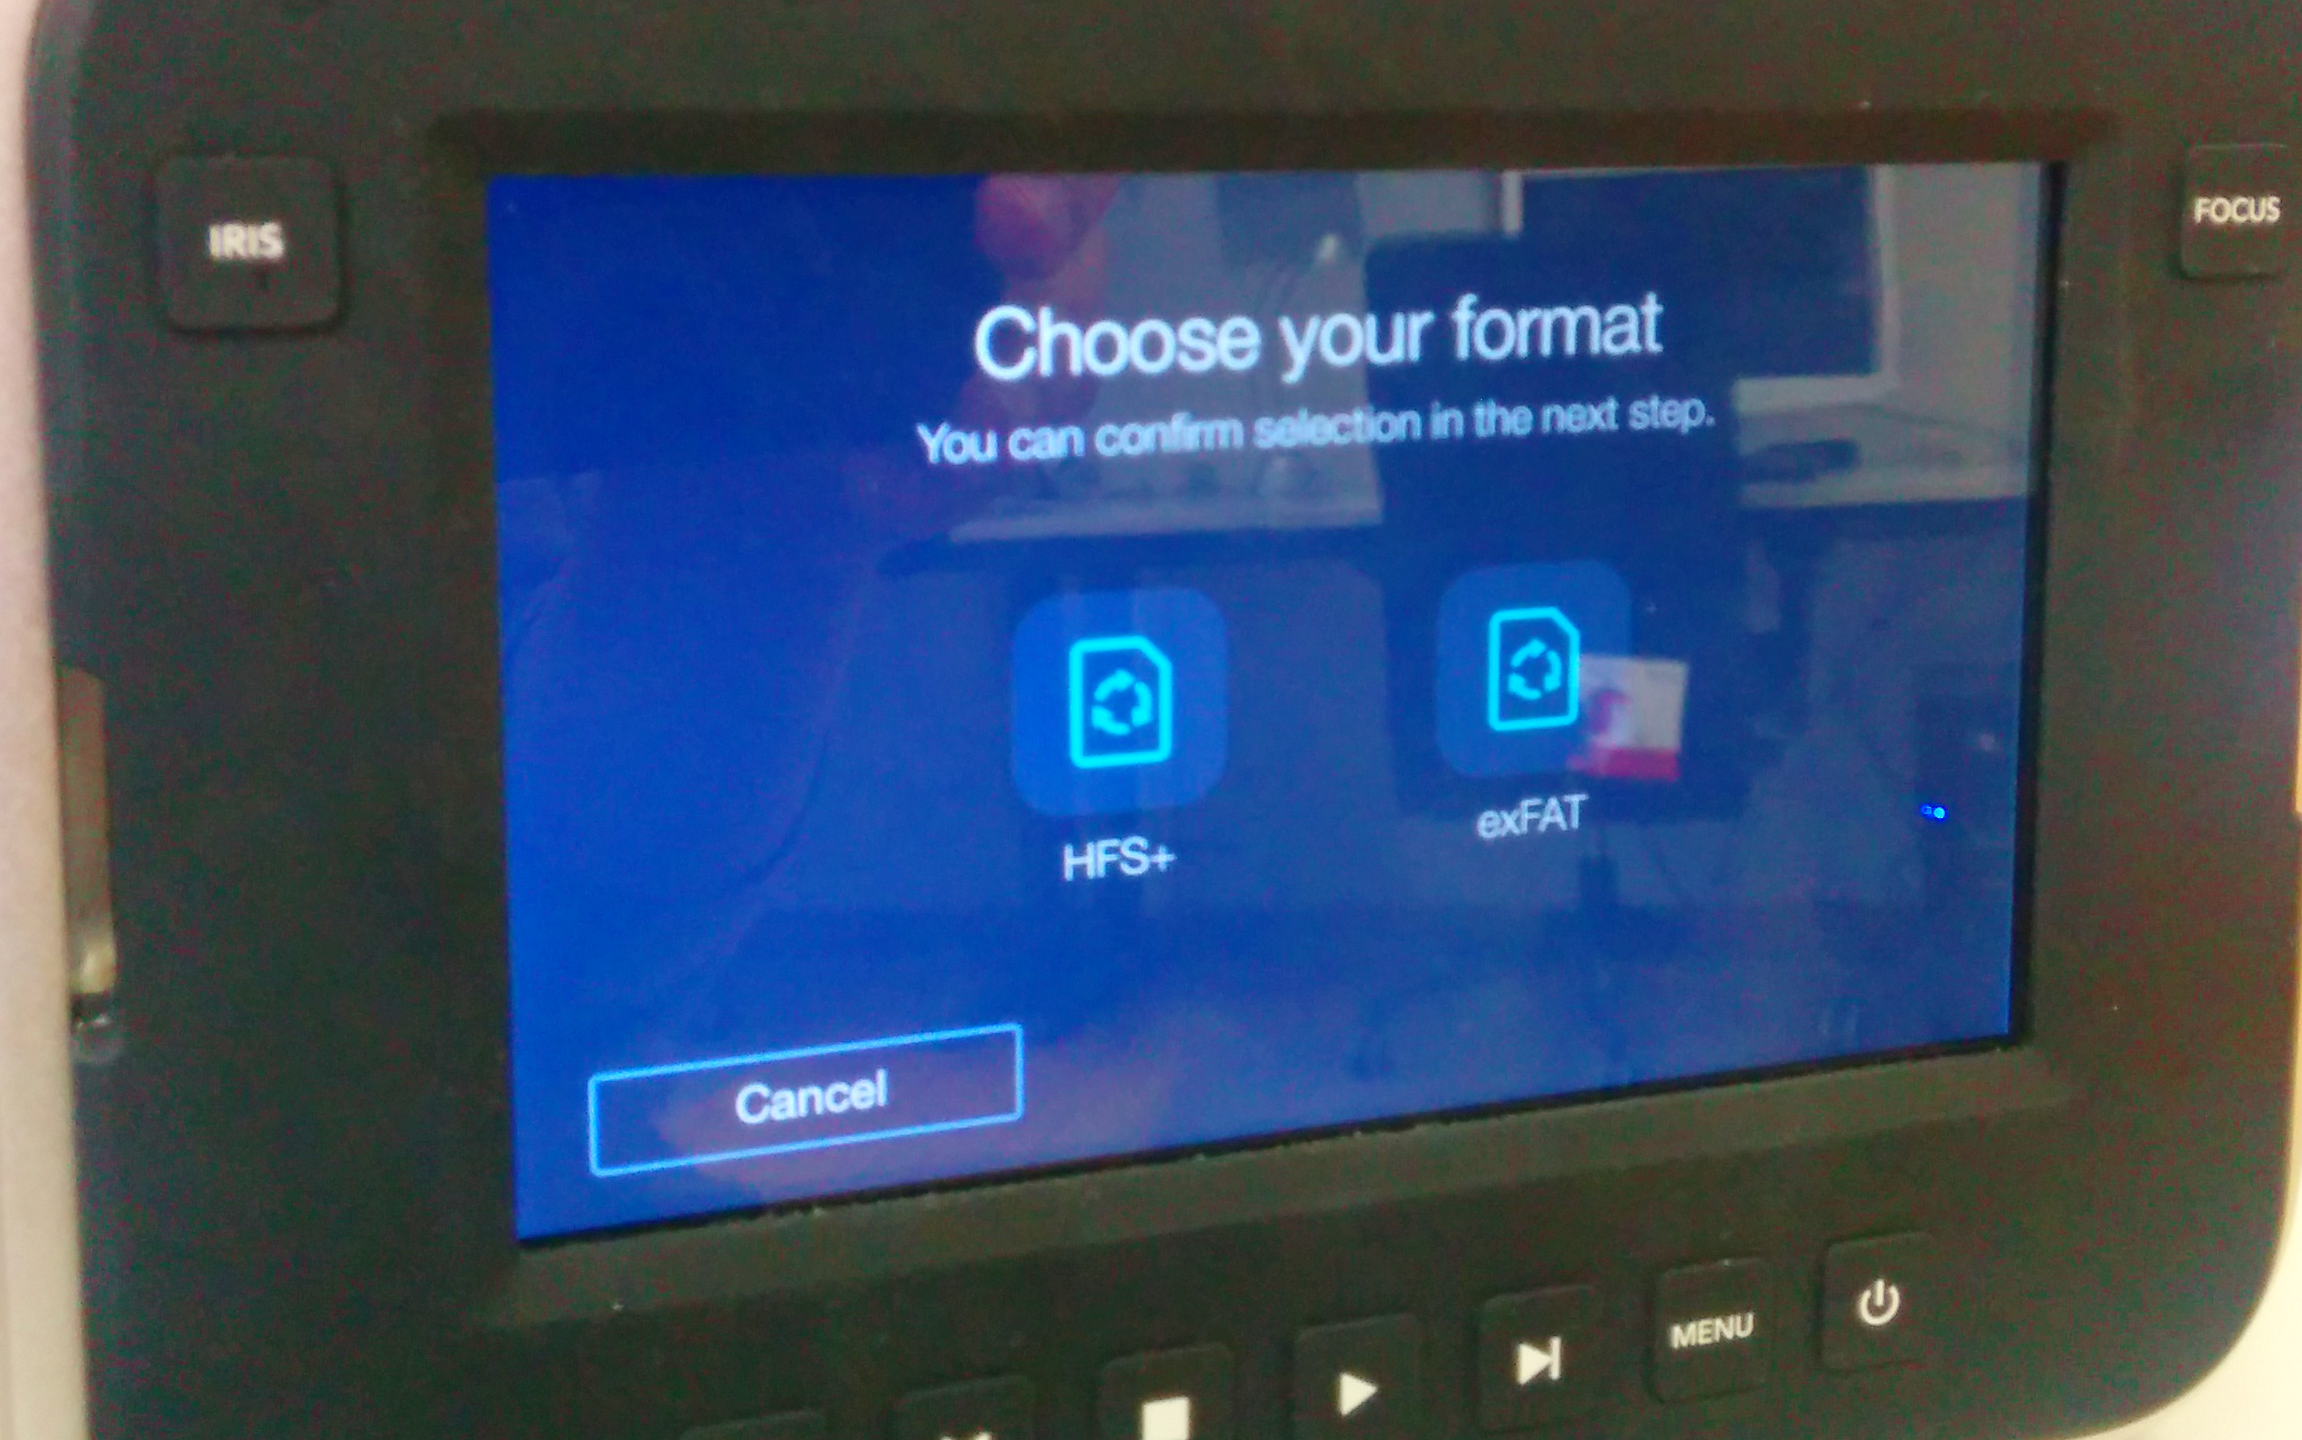
\includegraphics[width=\textwidth]{figures/camera1.png}
	      \caption{}
		\label{fig_cam_b}
	\end{subfigure}	        
	\begin{subfigure}[b]{0.22\textwidth}
	       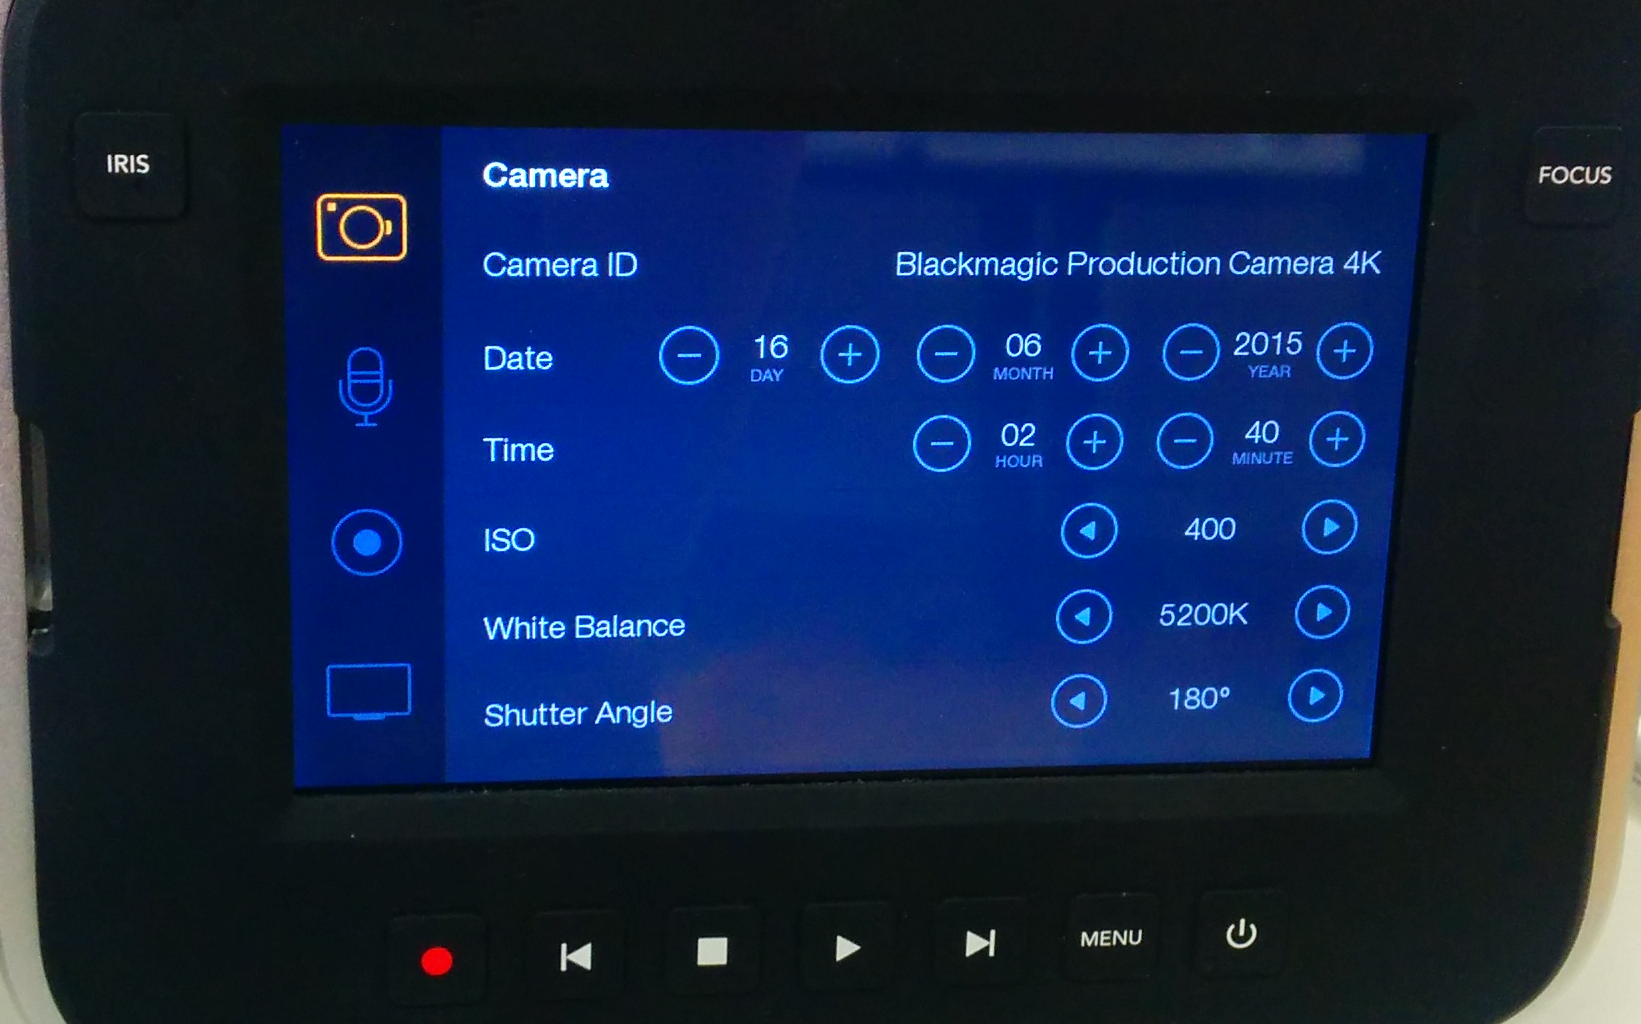
\includegraphics[width=\textwidth]{figures/camera3.png}
	       \caption{}
	\label{fig_cam_c}
	\end{subfigure}
	\begin{subfigure}[b]{0.22\textwidth}
	      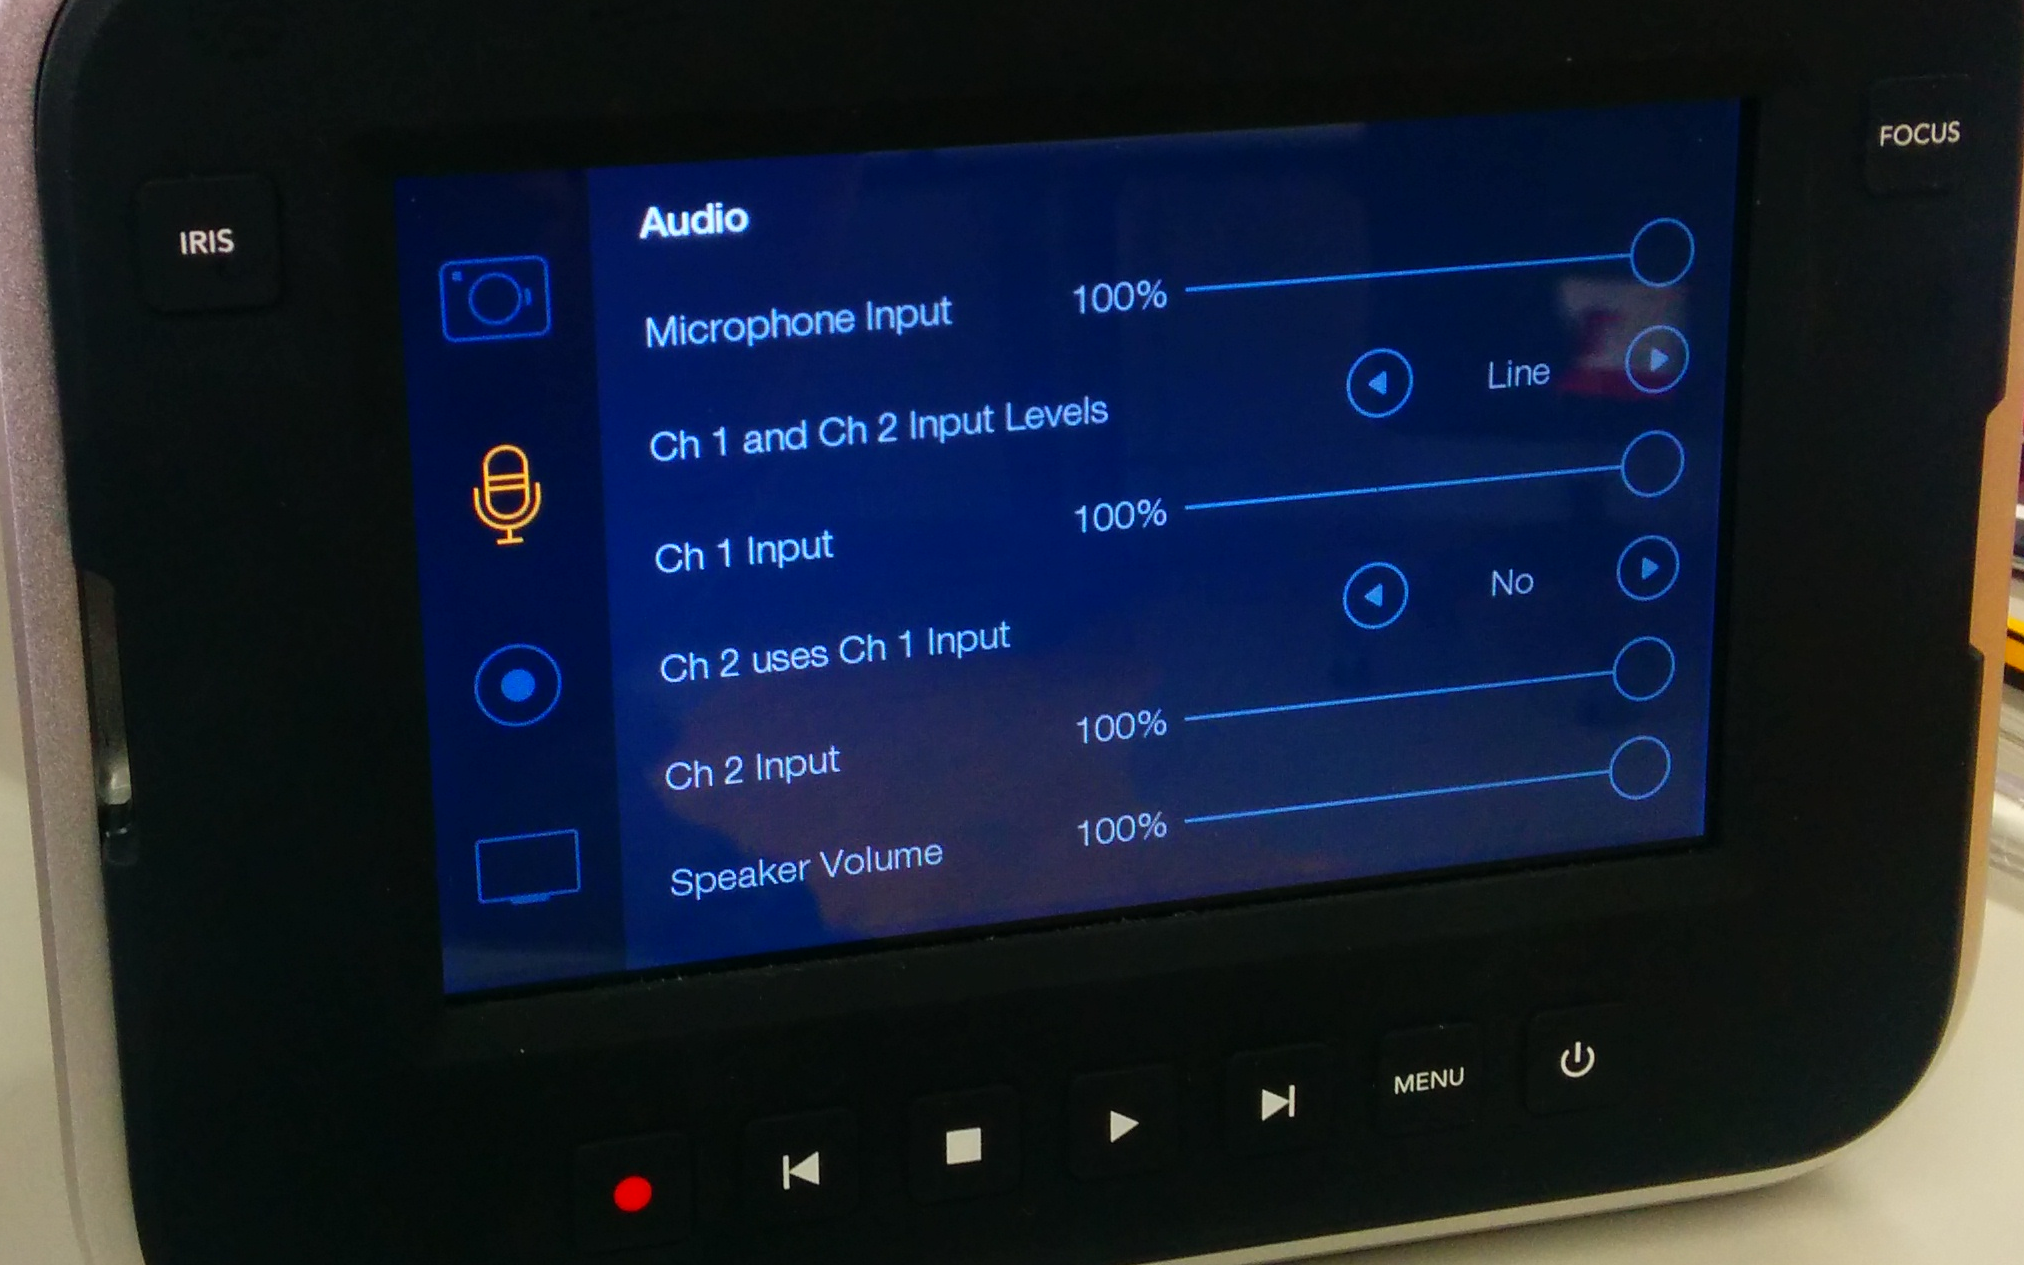
\includegraphics[width=\textwidth]{figures/camera4.png}
	      \caption{}
		\label{fig_cam_d}
	\end{subfigure}
	\begin{subfigure}[b]{0.22\textwidth}
	      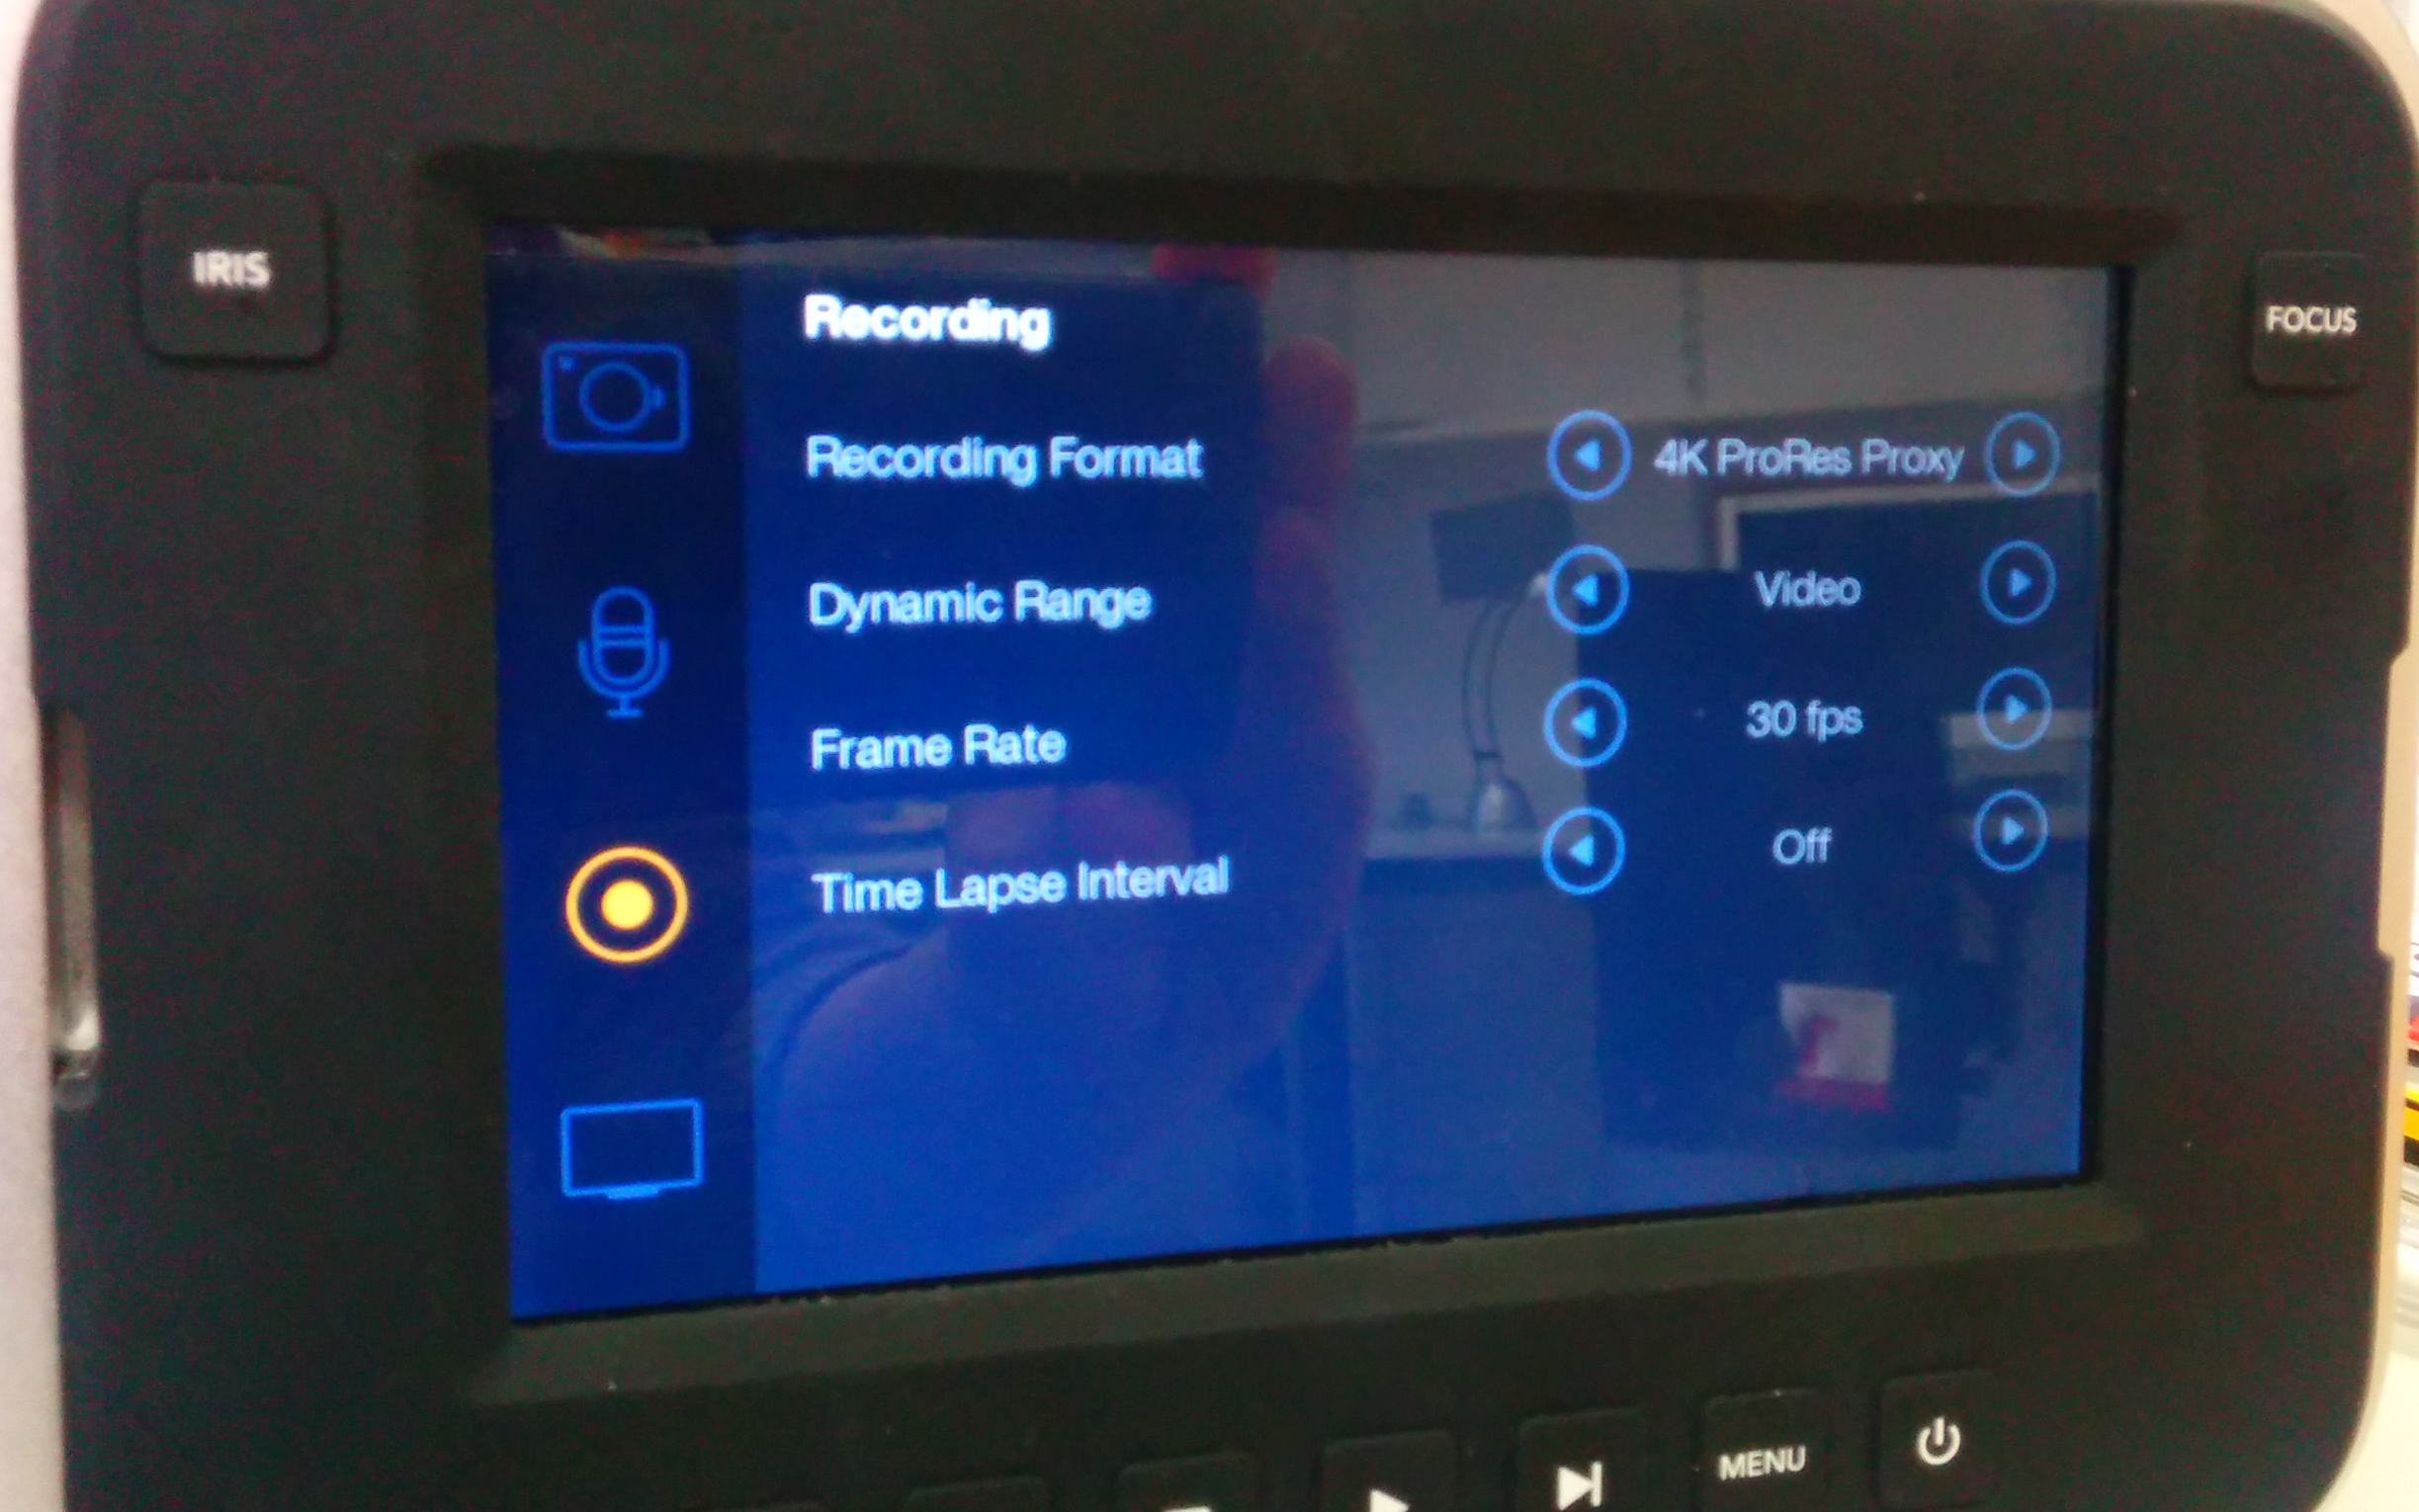
\includegraphics[width=\textwidth]{figures/camera5.png}
	      \caption{}
		\label{fig_cam_e}
	\end{subfigure}
	\caption{The setting menu of Blackmagic camera}
	\label{fig_cam}
\end{figure}


\subsection{ Camera Codec Formats}

The camera has 8 various recording formats as listed in table \ref{table_codecs}. After trying them, we reached the conclusion that base on the fact that the bit-depth of the video for all formats is 10 bits and according to the size, $PSNR$ values and video quality,  the \textbf{4k ProRes Proxy} was chosen to record the videos with 30 frame per second (fps). Moreover, different codings with the appropriate container have been examined as shown in table \ref{table_con}. One can compare the quality of coded videos. The \textbf{.mp4} container and \textbf{x264} coder might be selected as the most promising one for the final video.

\begin{table}[ht] 
		\centering % used for centering table 
		\caption{The different codecs of 4k Blackmagic camera } 	
		\label{table_codecs} 
		\begin{tabular}{llll} % centered columns (4 columns) 
			 \hline \hline
		Camera codec formats	&  Size (MB/sec) &  Size (GB/90 min) 	&  $PSNR$ \\ 
		\hline
		4k ProRes Proxy 	& 23.1		& 125	& 20 Db	\\
		4k ProRes LT  		& 51.6		& 279	&33 Db	\\
		4k ProRes 422  	& 74.0		& 400	&22 Db	\\
		4k ProRes HQ 		& 108.7		& 587	&99 Db	\\
		2k ProRes Proxy  	& 6.3		& 34		&32 Db	\\
		2k ProRes LT  		& 13.7		& 73		&37 Db	\\
		2k ProRes 422  	& 19.2		& 103	&33 Db	\\
		2k ProRes HQ  	& 28.0		& 151	&99 Db		  
		\end{tabular} 
	\end{table}


\begin{table}[H] 
		\centering % used for centering table 
		\caption{The different codecs of 4k Blackmagic camera versus different kind of containers and transcoders.
\ding{56} : bad quality , 
\ding{52} : good quality ,
\ding{50} : medium quality} 	
		\label{table_con} 
		\begin{tabular}{llllll} % centered columns (4 columns) 
			 \hline \hline
		Camera codec 	&  .webm   &  .mp4 	&   .mp4  &  .avi  & .agv \\ 
		formats	&  (vpx)  &  (x264)	&    (mpeg4) & (raw video)  & (theora) \\ 
		\hline
		4k ProRes Proxy 	&\ding{50}		& \ding{52}	& \ding{56}		&  \ding{56}	 & \ding{56}	\\
		4k ProRes LT  		&\ding{50}		& \ding{52}	& \ding{56}		&  \ding{56}	 & \ding{56}	\\
		4k ProRes 422  	&\ding{50}		& \ding{52}	& \ding{56}		&  \ding{56}	 & \ding{56}	\\
		4k ProRes HQ 		&\ding{50}		& \ding{52}	& \ding{56}		&  \ding{56}	 & \ding{56}	\\
		2k ProRes Proxy  	&\ding{56}		& \ding{50}	& \ding{56}		&  \ding{56}	 & \ding{56}	\\
		2k ProRes LT  		&\ding{56}		& \ding{52}	& \ding{56}		&  \ding{56}	 & \ding{56}	\\
		2k ProRes 422  	&\ding{50}		& \ding{52}	& \ding{56}		&  \ding{56}	 & \ding{56}	\\
		2k ProRes HQ  	&\ding{50}		& \ding{52}	& \ding{56}		&  \ding{56}	 & \ding{56}		  
		\end{tabular} 
	\end{table}



\section{Source Code}

\subsection{Code Hierarchy}

In this work, the Python language has been used to develop the methods. To access, follow, add and develop the source code, we have used the package and module hierarchy as follow. 

\vspace{1cm}


\dirtree{%
.1 SourceCode.
.2 demo.py.
.2 audio.
.3 audioProcessing.py.
.2 video.
.4 editing.
.5 layout.py.
.4 processing.
.6 CMT package.
.7 CMT.py.
.7 util.py.
.6 preProcessing.py.
.6 postProcessing.py.
.6 slideDetection.py.
.6 speakerTracking.py.
.2 util.
.5 templateMatching.py.
.5 tools.py.
}

\vspace{1cm}



\begin{figure}[H]
\resizebox{1\linewidth}{!}{
\pgfdeclarelayer{background}
\pgfdeclarelayer{foreground}
\pgfsetlayers{background,main,foreground}

\begin{tikzpicture}[>=latex']

\tikzset{block/.style={
      rectangle,
      draw=blue,
      thick,
      fill=gray!20,
      text width=3cm,
      align=center,
      rounded corners,
      minimum height=2em
    },
bigblock/.style={
      rectangle,
      draw=blue,
      thick,
      fill=gray!20,
      text width=5cm,
      align=center,
      rounded corners,
      minimum height=2em
    },
    oblock/.style={
          rectangle,
          draw=blue,
          thick,
          fill=gray!20,
          text width=2.7cm,
          align=center,
          rounded corners,
          minimum height=2em
        }, 
rblock/.style={draw, shape=rectangle,rounded corners=1.5em,align=center,minimum height=4cm, text centered, text width= 3cm},
database/.style={draw, shape=cylinder, cylinder uses custom fill,
      shape border rotate=90, aspect=0.25,text centered, text width= 2.5cm, minimum height=3cm, fill=gray!20,
      draw=blue},
ann/.style= {above, text width=10em, text centered},
}


\node[inner sep=0pt] (video)  at (0,0) 
    { 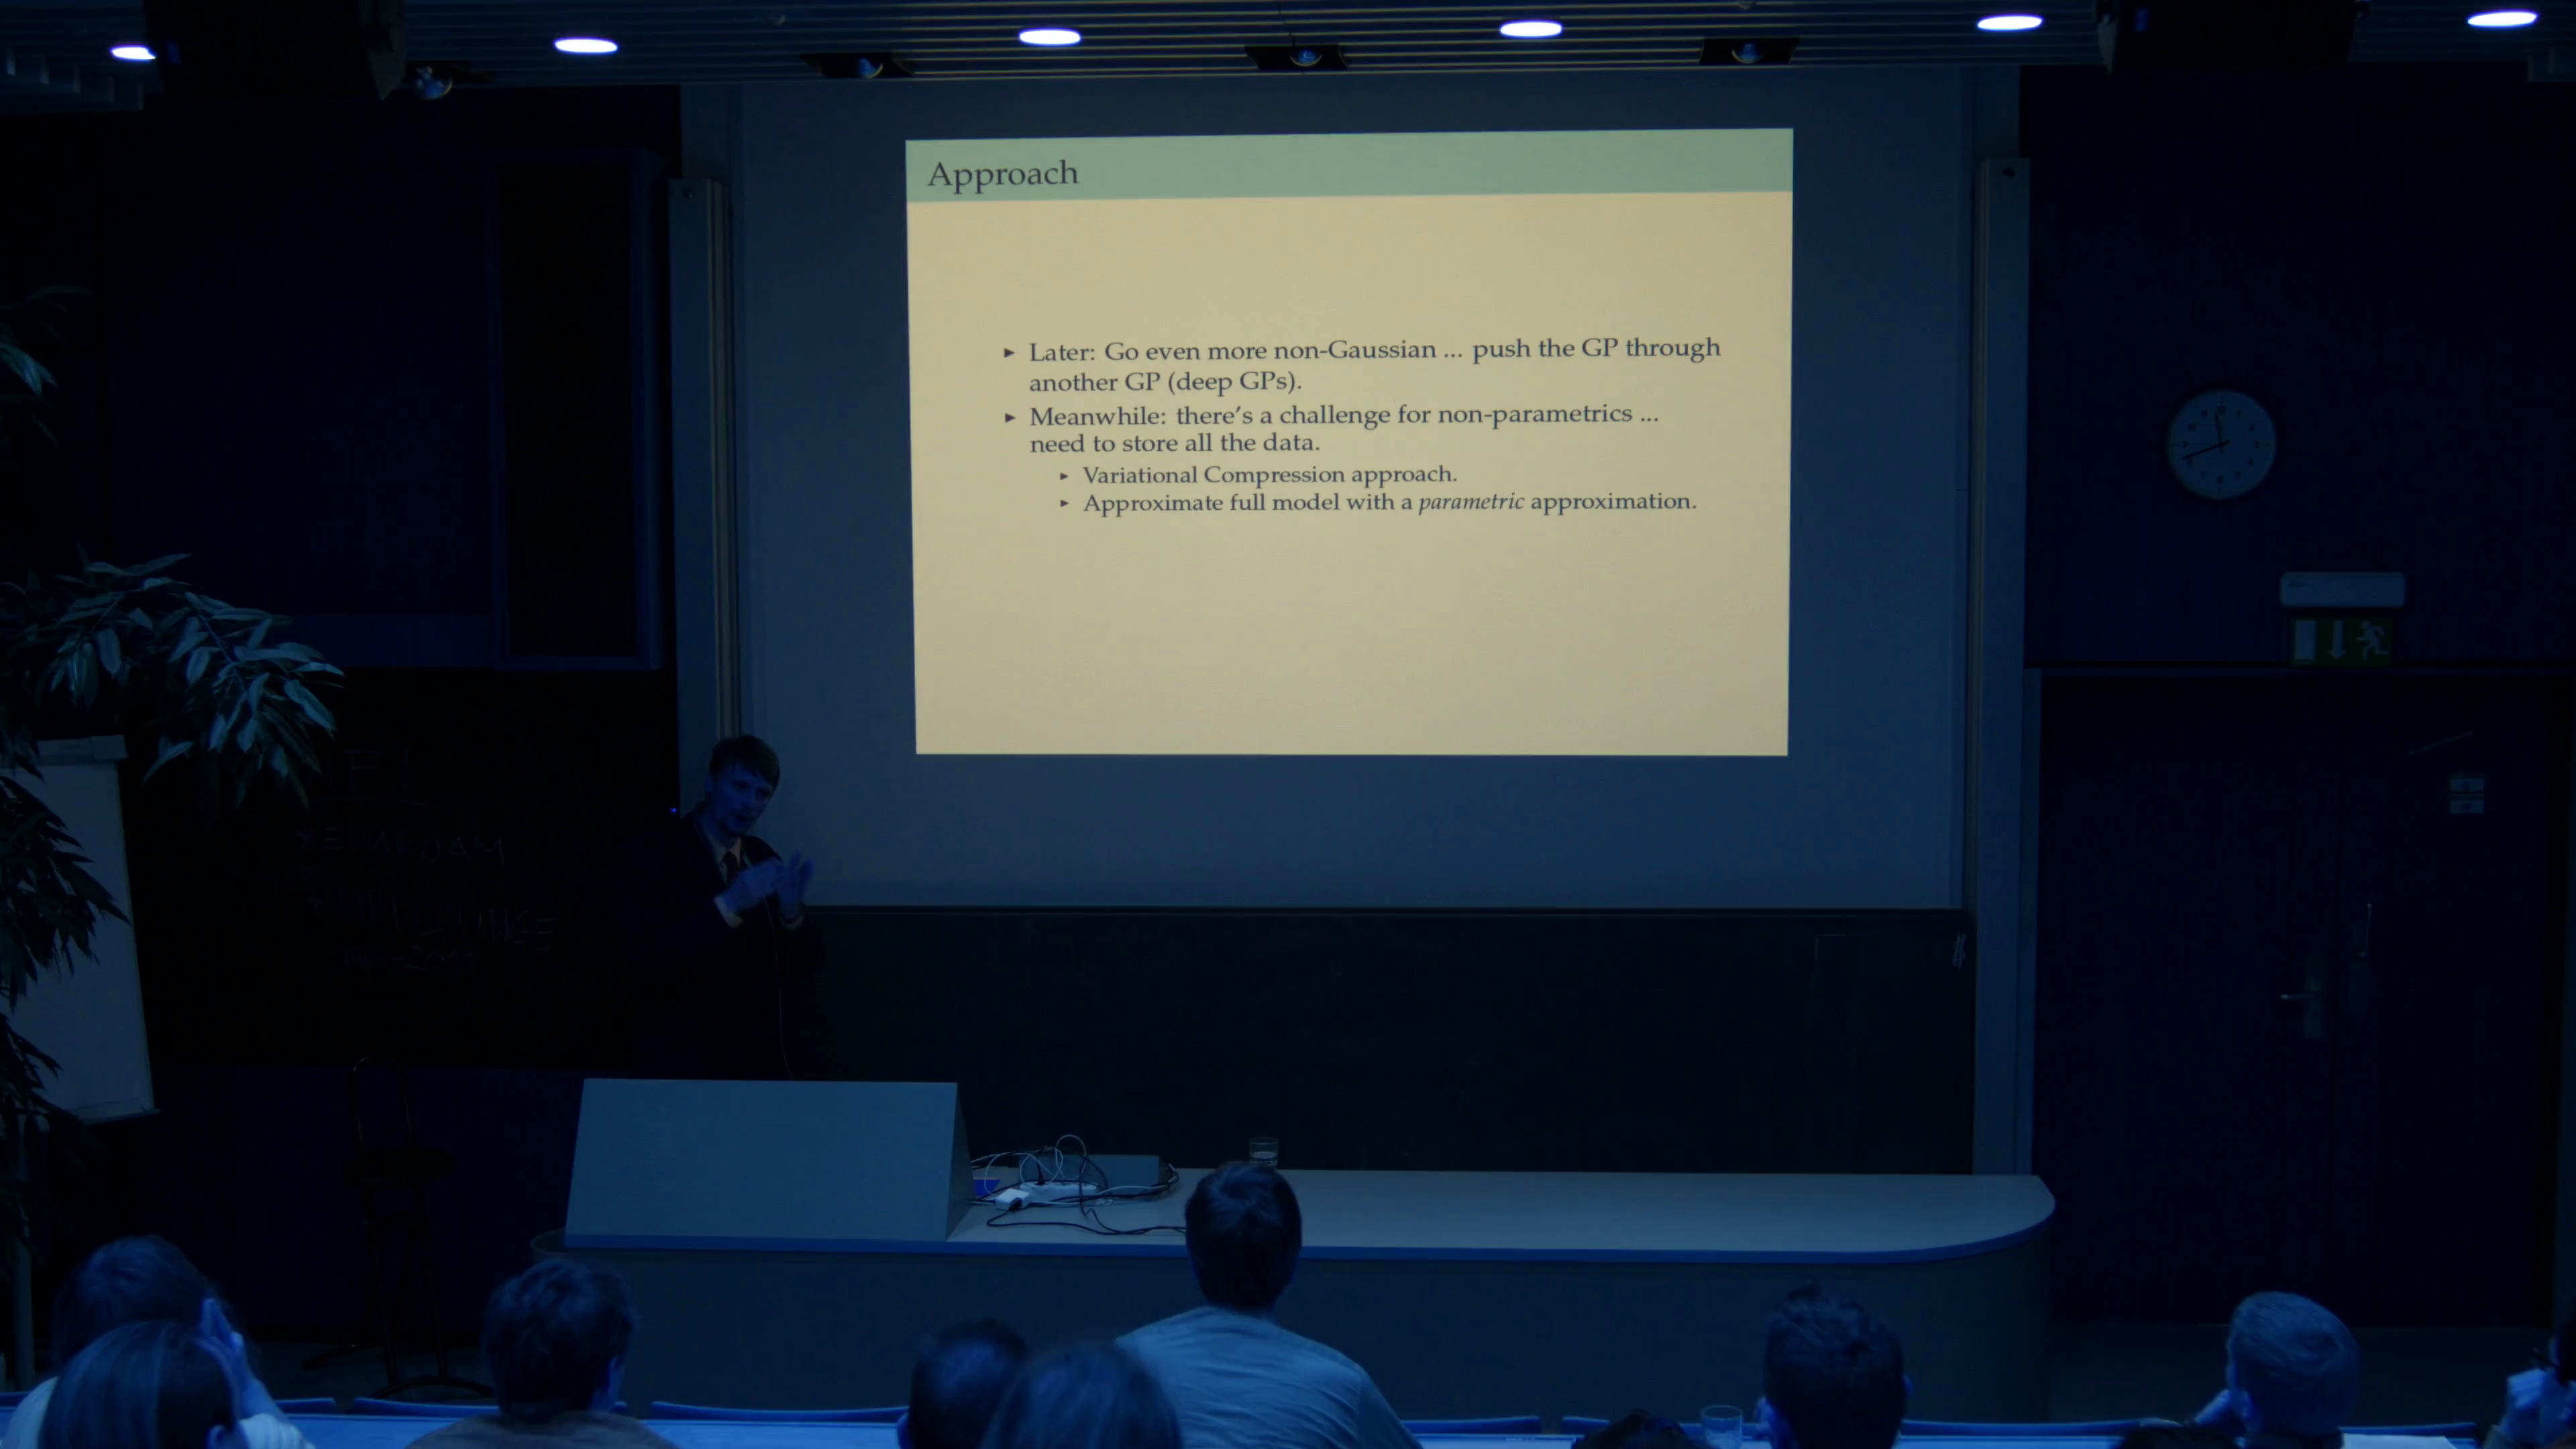
\includegraphics[width=0.15\textwidth]{figures/video.png}};

\node [block, above right =1cm of video]  (vp1) {preProcessing.py};
\node [block, above right  = 0.3cm of vp1]  (vp2) {slideDetection.py};
\node [block, below =1.5cm of vp2]  (vp3) {speakerTracking.py};
\node [block, right =3cm of vp1]  (vp4) {postProcessing.py};
\node [block, right =1cm of vp4]  (ve5) {layout.py};
\node [block, right =0.5cm of ve5]  (ve6) {layout.py};
\node[inner sep=0pt,  below right =1cm of ve6] (layout)  { 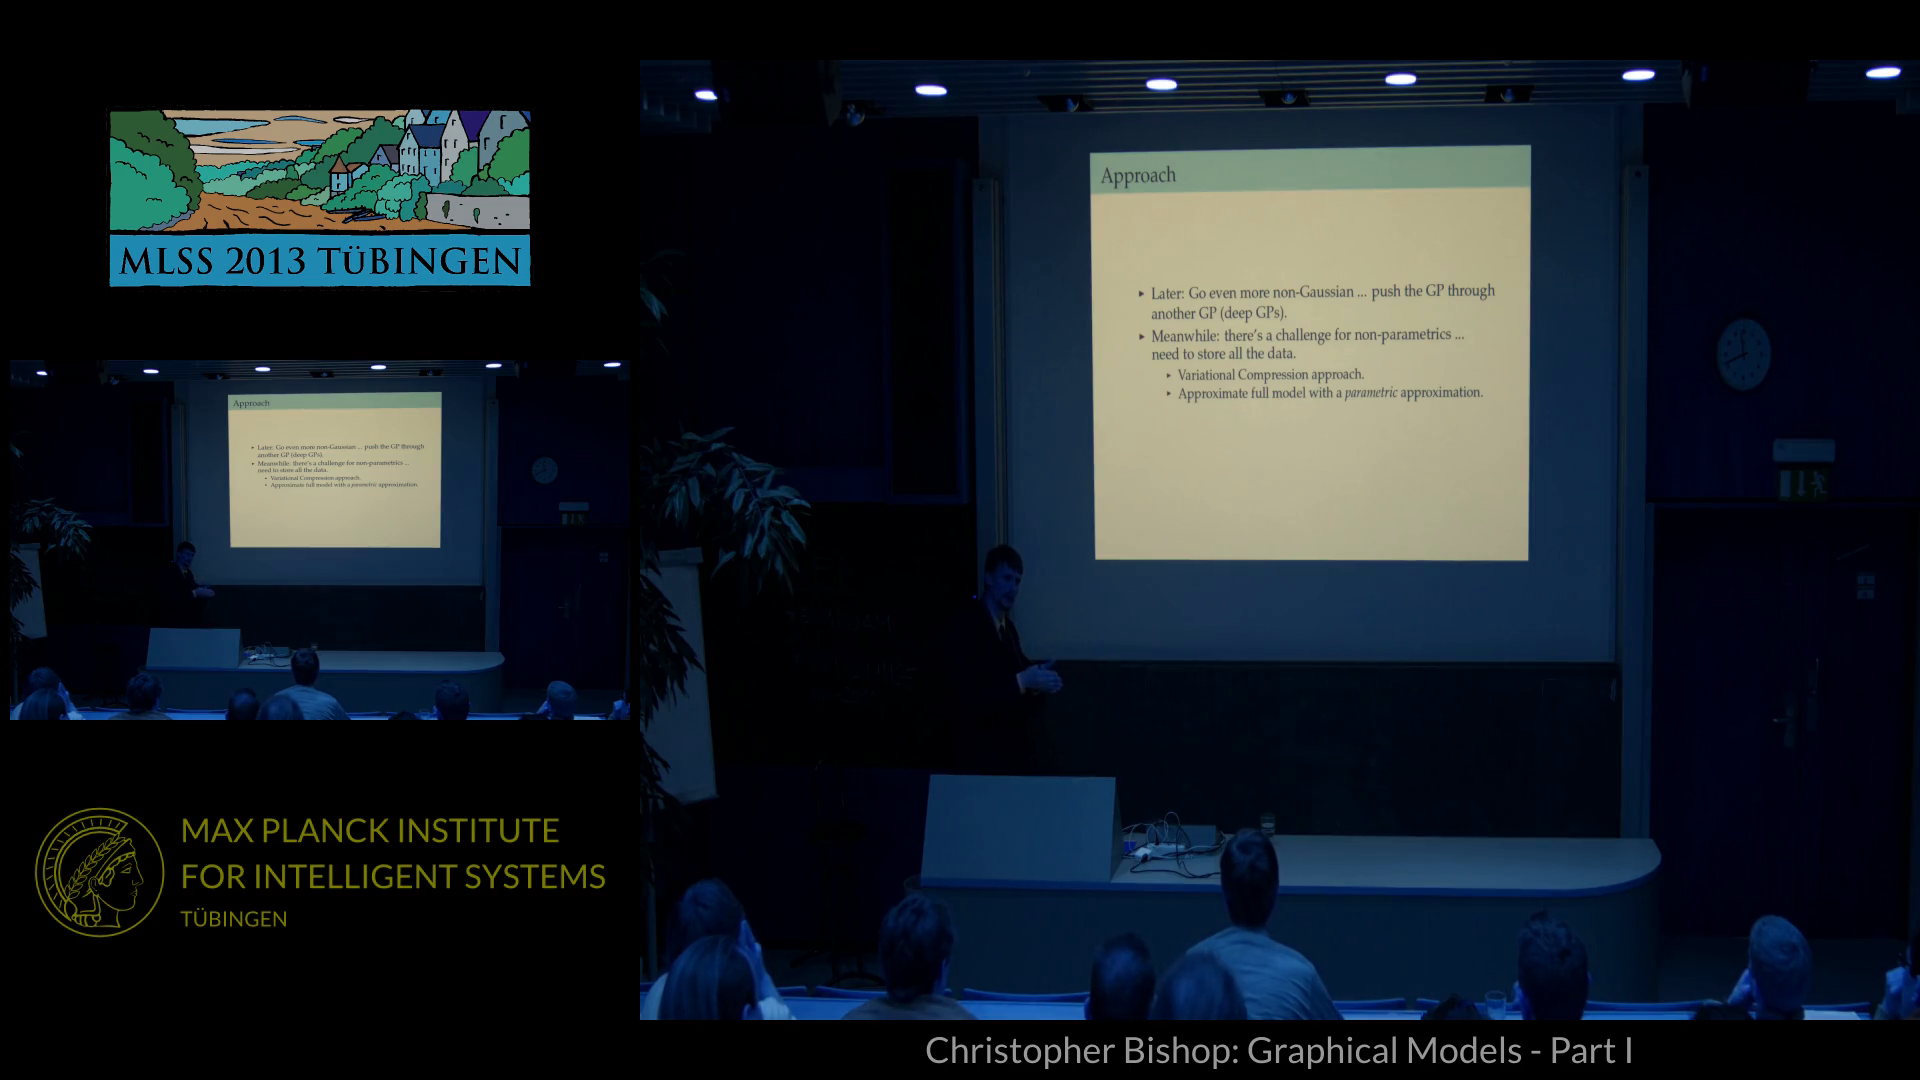
\includegraphics[width=0.15\textwidth]{figures/layout.png}};

\node [bigblock, below=4cm of vp4]  (ap1) {audioProcessing.py};


\node [ann, below right=1cm of vp4]  (bk) {Background Image};
\node [ann, below =0.01cm of bk]  (info) {Talk/Speaker Info.};

\begin{pgfonlayer}{background}
        \path (vp1.west |- vp2.north)+(-0.3,0.3) node (a) {};
        \path (vp3.south -| vp4.east)+(0.3,-0.3) node (b) {};       
        \path[fill=blue!10,rounded corners, draw=black!50, dashed]
            (a) rectangle (b);           
        \path (vp2.north)+(0.0,+0.5) node (a) {processing Package};            
 \end{pgfonlayer}


\begin{pgfonlayer}{background}
        \path (ve5.west |- ve5.north)+(-0.3,0.3) node (a) {};
        \path (ve6.south -| ve6.east)+(0.3,-0.3) node (b) {};       
        \path[fill=blue!10,rounded corners, draw=black!50, dashed]
            (a) rectangle (b);           
        \path (ve5.north east)+(0.0,+0.5) node (a) {editing package};            
 \end{pgfonlayer}


\begin{pgfonlayer}{background}
        \path (ap1.west |- ap1.north)+(-0.5,0.5) node (a) {};
        \path (ap1.south -| ap1.east)+(0.5,-0.5) node (b) {};       
        \path[rounded corners, draw=black!150, dashed]
            (a) rectangle (b);           
        \path (ap1.north)+(0.0,+0.7) node (a) {audio package};            
 \end{pgfonlayer}


\begin{pgfonlayer}{background}
        \path (vp1.west |- vp2.north)+(-0.7,0.7) node (a) {};
        \path (vp3.south -| ve6.east)+(0.7,-0.7) node (b) {};       
        \path[rounded corners, draw=black!150, dashed]
            (a) rectangle (b);           
        \path (vp4.north)+(0.0,+2.1) node (a) {video Package};            
 \end{pgfonlayer}



 paths
\path[draw,->] 
          	(vp1) edge (vp2)
          	(vp1) edge (vp3)
	 	(vp3) edge (vp4)
	  	(vp2) edge (vp4)
		(vp4) edge (ve5)
		(ve5) edge (ve6)

;
               
\draw[-latex] +(1,1.5) node (a) {video }(video.east) -- ++(0.5,0)  |-  (vp1.west) ;
\draw[-latex] +(1,-1.5) node (a2) {audio }(video.east) -- ++(0.5,0) |-  (ap1.west);

\draw[-latex] (ve6.east) -- ++(0.5,0) |-  (layout.west);
\draw[-latex] (ap1.east) -- ++(3.4,0) |-  (ve6.west);

\draw[-latex] (bk.west) -- ++ (-0.2,0.0) |-  (ve5.west);
\draw[-latex] (info.west) -- ++(-0.2,0.0) |-  (ve5.west);


\end{tikzpicture}
}
\vspace{-0.3cm}
    \caption{\small The name of the modules in the framework.}
    \label{fig_framework}
\centering
\end{figure}



The main folder is the \lq\lq SourceCode\rq\rq which includes a file \texttt{demo.py}. This file is to run the whole framework. One can simply specify the path to the input video, the path to the input background image, add some comments as the information of talk as the input arguments and get the final video with the corresponding sound. Here the audio file does not modify.

According to figure \ref{fig_framework}, the input file will be extracted into audio and video parts. For each part, one package is defined, i.e. two packages (\lq\lq audio\rq\rq and \lq\lq video\rq\rq) are defined. Furthermore, it has a package named \lq\lq util\rq\rq composed of all methods for the utilities. If you intend to add any methods for secondary implementations, please add it into \texttt{tools.py} or simply write a module and put it inside the \lq\lq util\rq\rq package like \texttt{templateMatching.py}.

The \lq\lq audio\rq\rq package is composed of the \texttt{audioProcessing.py} module in which one may add some methods/classes for audio analyses (For now, it is empty).

The \lq\lq video\rq\rq package is composed of two sub-packages (editing and processing) as shown in figure \ref{fig_framework}.  \lq\lq editing\rq\rq has one module named \texttt{layout.py} to form the final layout, concatenate the audio file and write the final video. \lq\lq processing\rq\rq is composed of four modules such as \texttt{preProcessing.py} , \texttt{postProcessing.py}, \texttt{slideDetection.py} and \texttt{speakerTracking.py} and different number of sub-packages like \lq\lq CMT\rq\rq that contains all files for the corresponding algorithm. If you need to use a ready written package for video processing, simply put it in the folder \lq\lq processing\rq\rq.

\begin{itemize}
\item preProcessing: It can be considered as a module to have all pre -processing functions such as segmentation, contrast enhancement and so on.

\item slideDetection: This module implements various algorithms for slide detection. For each algorithm, 
one class has been defined in which there is a method named \textit{slideDetector} to call.
Different classes have different attributes, but in order to call the corresponding function \textit{slideDetector}, all classes are the same. It includes the following classes.

\begin{enumerate}
\item templateMatch
\item connectedComponent
\item polygonDetection
\item harrisCornerDetection
\item getUserCropping
\end{enumerate}

\item speakerTracking: This module implements various algorithms based on CMT for speaker tracking. 
This algorithm has been combined with Kalman filter, and 
different approaches have been used to ease the computation time.
 For every algorithm, one class has been defined in which there is a method named \textit{speakerTracker} to call.
Different classes have different attributes, but in order to call the corresponding
function \textit{speakerTracker}, all classes are the same. It includes the following classes.

\begin{enumerate}
\item \texttt{CMT\_algorithm}
\item \texttt{CMT\_algorithm\_kalman\_filter}
\item \texttt{CMT\_algorithm\_kalman\_filter\_stripe}
\item \texttt{CMT\_algorithm\_kalman\_filter\_downsample}
\item \texttt{CMT\_algorithm\_kalman\_filter\_no\_vertical}
\item \texttt{CMT\_algorithm\_kalman\_filter\_downsample\_no\_vertical}
\item \texttt{FOV\_specification}
\end{enumerate}

\item postProcessing: All functions for post-processing like \textit{perspective\_transformation}

In the next section, a short overview of main tasks will be discussed.

\end{itemize}

\subsection{Slide Detection}

\subsection{Speaker Tracking}


\subsubsection{CMT}
Speaker tracking is still an unsolved problem due to various type of changes, poses, appearances and local and global illumination changes. In our work, we use one of the most promising algorithms named \lq\lq Consensus-based tracking and matching of the keypoints \rq\rq or so called CMT. As a short introduction of CMT, one has to mention that it is a free-model object tracking in a combination of both matching and tracking framework. It does not need a specific knowledge  and training samples. 

In CMT, the object of interest (ex. the speaker) is selected in the first frame and some keypoints are extracted. It is possible to use different detectors, descriptors such as SIFT/SURF, ORB, Brisk, etc to obtain the keypoints. In the downloaded version of CMT, the Brisk detector and descriptor are used. After obtaining all of the desired keypoints corresponding to the object of interest, the main idea is to again find the keypoints which were already included in the initial selection. This progress is done by employing two different steps.

\begin{enumerate}

\item It tracks the keypoints from previous frame to the current frame by estimating optical flow.
\item They match the keypoints by comparing their descriptors.
\item In each frame, in order to localize the object of interest, a voting factor is used to vote and compute the center of the object.
\item Finally, a consensus scheme is applied to remove the outliers and keep the related keypoints.
\end{enumerate}

Let's assume, we have a sequence of the frames (from $I_1$ to $I_n$) and the desire object of interest inside the first frame. As you can see in the table, it is called $b_1$. 
So, the output is to find the selected object inside all of the next frames ($b_2$ to $b_n$). Then, by means of Brisk detector, the keypoints will be computed as well as the corresponding descriptors. We assign all of the desired keypoints which we want to look for them through the whole frames into $O$ set. It means, $O$ includes all of the keypoints of the object of interest. After that, for all of the frames (from 2nd to n-th), the candidate keypoints are computed so that they can be inside or outside the region of interest. Hence, $P$ is a set composing of all candidate keypoints. For each of the $P$'s member, the hamming distance between their descriptor and the descriptor of desired keypoints are calculated and matched by means of nearest-neighbor matcher. The results will be put into $M$. In order to track the keypoints, we compute the displacement of them from frame $I_{t-1}$ and $I_{t}$ by Lucas and Kanade method for estimating the optical flow. Afterwards, to discard all tracked keypoints which are matched as well, we fuse $T$ and $M$ keypoints and form the set of keypoints names $K$. Due to some failure in the tracking and matching progress, $K$ can be included the outliers. Therefore, one voting factor is used to estimate the center of object and a consensus-based method is applied to eliminate the outliers. In this case, the votes are clustered based on euclidean distance and a threshold value and then the consensus voting will be identified based on the highest number of votes. The votes inside the consensus cluster are kept and the remaining will be prone out. As an output of CMT for each frame, the mean value of the center of the object calculated by voted keypoints are extracted. Then, this loop will be continued till the last frame \cite{nebehay2014consensus}. The whole CMT algorithm can be summarized as follow:


\begin{enumerate}

\item Initialise detector, descriptor, matcher
\item Get initial keypoints in whole image (first frame)
\item In each frame, in order to localize the object of interest, a voting factor is used to vote and compute the center of the object.
\item Finally, a consensus scheme is applied to remove the outliers and keep the related keypoints.
\end{enumerate}



\begin{itemize}


  \item Getting user's object of interest: (function:  \texttt{get\_rect} in \texttt{util} module in \texttt{CMT} package)
  \begin{enumerate}
    \item It reads the first frame and get the rectangle input from the user.
  \end{enumerate}

\item Initialization:  (function: \texttt{initialise} in \texttt{CMT} module in \texttt{CMT} package)
  \begin{enumerate}
    	\item Initialise detector, descriptor, matcher
  	  \item Get initial keypoints in whole image
	\item Remember keypoints that are in the rectangle as selected keypoints and those which are not in the rectangle as background keypoints
	\item Assign each keypoint a class starting from 1, background is 0
	\item Get all distances between selected keypoints by calculating square root and compute all angles between selected keypoints
	\item Compute the vector from the first keypoint (k1) to the 2nd keypoint (k2)
	\item Compute angle of this vector with respect to x axis and store it
	\item Find the center of selected keypoints as the mean of all selected keypoints
  \end{enumerate}


  \item Tacking and Matching: (function: \texttt{process\_frame} in \texttt{CMT} module in \texttt{CMT} package), These steps are sequentially repeated for all frames
  \begin{enumerate}
    	\item Detect keypoints, compute descriptors and get all matches for selected features
	\item Track the keypoints between the previous and current frame by means of optical flow method. (function: \texttt{track} in \texttt{util} module in \texttt{CMT} package)

\begin{enumerate}
    	\item Calculate forward optical flow and backward optical flow for previous location
   	 \item Calculate forward-backward error
	\item Set status depending on the calculated error
  \end{enumerate}

	\item Estimate the parameters for matching and voting. (function: \texttt{estimate} in \texttt{CMT} module in \texttt{CMT} package)

\begin{enumerate}
    	\item Get all combinations of keypoints and measure distance between all
   	 \item Estimate the votes regarding one formula and remember all votes including outliers
	\item Compute pairwise distance between votes
	\item Compute linkage between pairwise distances
	\item Perform hierarchical distance-based clustering
	\item Count votes for each cluster and get largest cluster
	\item Identify members of largest class and compute the object center as a mean of all members
	\item Remember outliers and stop to track them
  \end{enumerate}

    \item For each keypoint and its descriptor

\begin{enumerate}
    	\item Retrieve keypoint location
   	 \item First: Match over whole image
	\item Compute distances to all descriptors
	\item Extract class of best match and add keypoint to active keypoints
	\item Add all tracked keypoints that have not been matched
	\item Update object state estimate
 \end{enumerate}

  \end{enumerate}

\end{itemize}







\section{Acknowledgments}

I would like to express my very great appreciation to all of team members, Michael Hirsch, Senya Polikovsky, Edgar Klenske, Michael Schober and Parnia Bahar for their patient, valuable and constructive suggestions during this research work.

% -------------------> end writing here <------------------------
% *****************************************************************
\clearpage

\bibliography{refs}
\bibliographystyle{ieeetr}
\end{document}